\documentclass[xcolor=dvipsnames]{beamer}
\usepackage[T1]{fontenc}
\usepackage[utf8]{inputenc}
\usepackage[english,slovak]{babel}

\usepackage{amsmath}
\usepackage{amsthm}
\usetheme{Pittsburgh}
\useoutertheme{shadow}

\usepackage{graphicx}
\usepackage{caption}
\usepackage{subcaption}

\usepackage[]{algorithm2e}
\usepackage{listings}
 \setbeamercovered{transparent}
 \usepackage{cuted}
\usepackage[export]{adjustbox}
\usepackage{mathtools}

\usepackage{lipsum}
\usepackage{verbatim}
\usepackage{transparent}
\usepackage{framed}
\usepackage{xcolor}

\usepackage{multirow}
\usepackage{colortbl}
\usepackage{lmodern}

\usepackage{movie15}
\usepackage{media9}
\usepackage{verbatim}

\usepackage{animate}


\usepackage{hyperref}

\newcommand\Wider[2][3em]{%
\makebox[\linewidth][c]{%
  \begin{minipage}{\dimexpr\textwidth+#1\relax}
  \raggedright#2
  \end{minipage}%
  }%
}






\iffalse

\usetheme{Warsaw}

\setbeamercolor{normal text}{fg=white,bg=black!90}
\setbeamercolor{structure}{fg=white}

\setbeamercolor{alerted text}{fg=red!85!black}

\setbeamercolor{item projected}{use=item,fg=black,bg=item.fg!35}

\setbeamercolor*{palette primary}{use=structure,fg=structure.fg}
\setbeamercolor*{palette secondary}{use=structure,fg=structure.fg!95!black}
\setbeamercolor*{palette tertiary}{use=structure,fg=structure.fg!90!black}
\setbeamercolor*{palette quaternary}{use=structure,fg=structure.fg!95!black,bg=black!80}

\setbeamercolor*{framesubtitle}{fg=white}

\setbeamercolor*{block title}{parent=structure,bg=black!60}
\setbeamercolor*{block body}{fg=black,bg=black!10}
\setbeamercolor*{block title alerted}{parent=alerted text,bg=black!15}
\setbeamercolor*{block title example}{parent=example text,bg=black!15}

\fi



%-------------------------------------------------------------------------------------
\title{\color{white} \bf Advanced reinforcement learning}
\author{\color{white} Michal CHOVANEC, PhD}


%\setbeamertemplate{footline}[frame number]{}
\setbeamertemplate{navigation symbols}{}


\date[EURP]{}
\begin{document}

{
    \usebackgroundtemplate
    {
        \vbox to \paperheight{\vfil\hbox to \paperwidth{\hfil

        {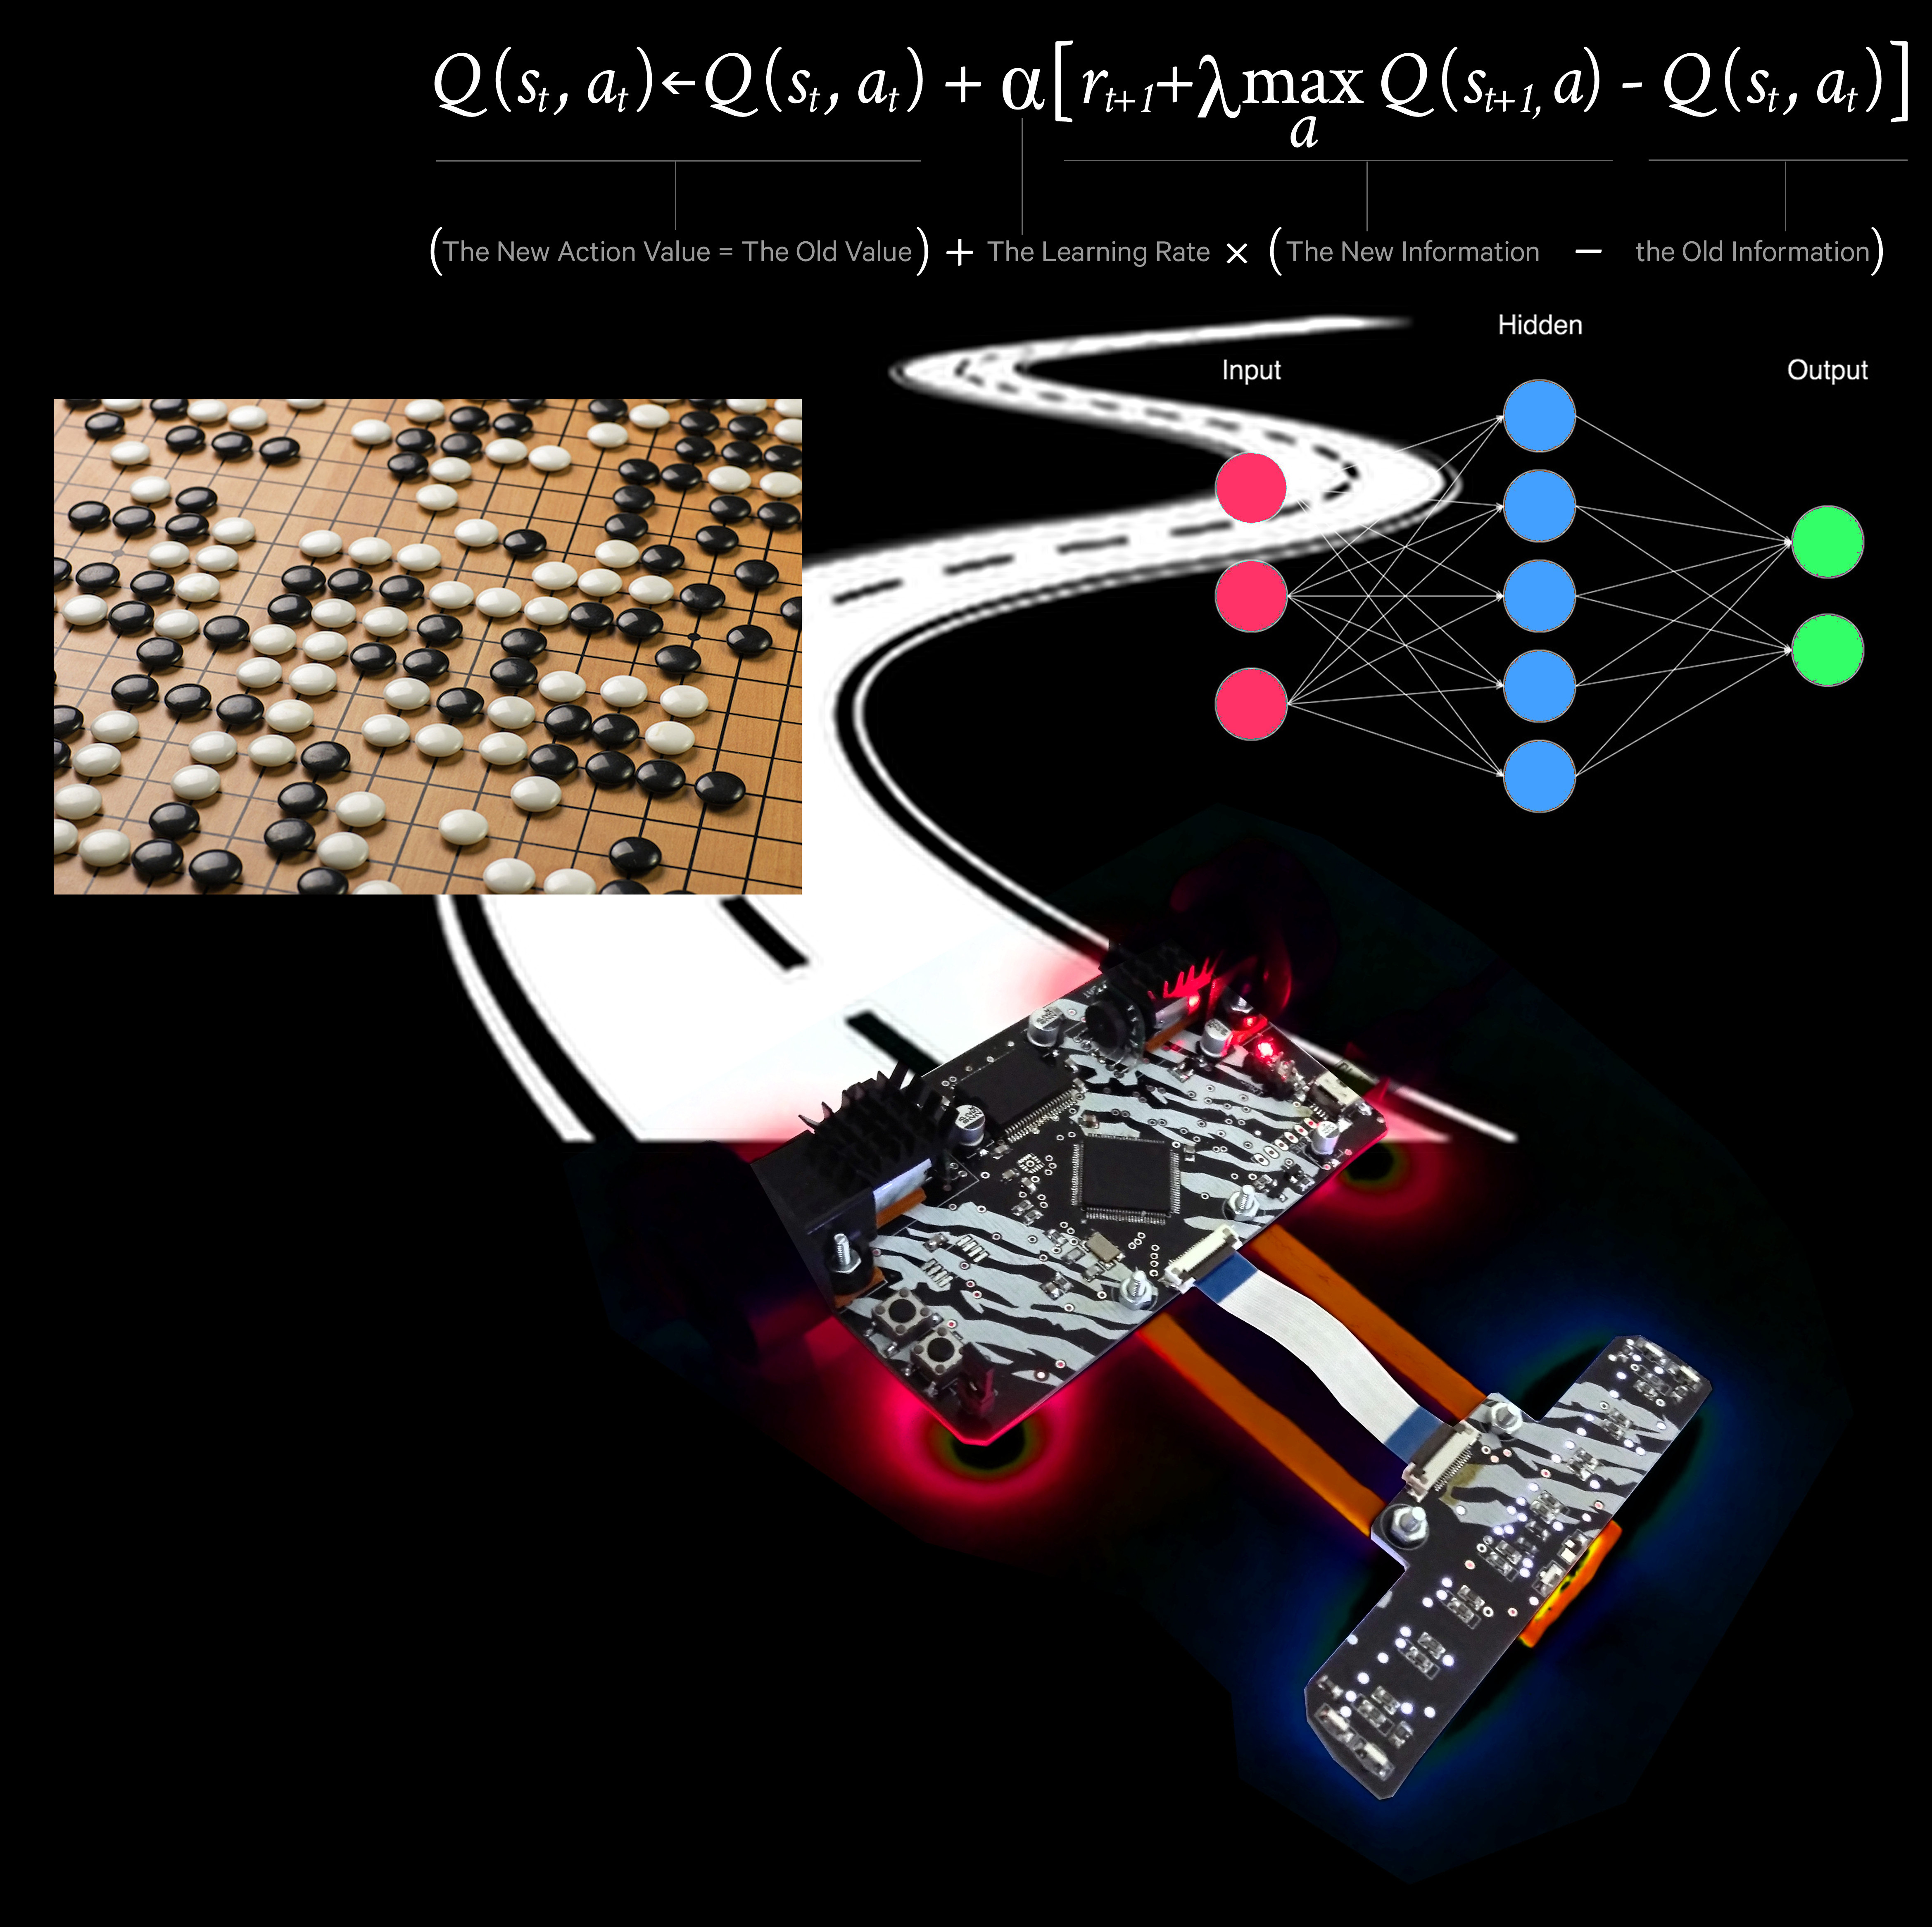
\includegraphics[width=5.05in]{../images/rl_square.jpg}}

        \hfil}\vfil}
    }



    \begin{frame}

    \centering
     \colorbox{black}
     {
        \begin{minipage}{7cm}
           {\LARGE \color{white} advanced RL} \\
           {\Large \color{white} - continuous controll \\- curiosity \\- imagination} \\
           {\LARGE \color{white} Michal CHOVANEC} \\
       \end{minipage}
     }

    \end{frame}
}

\begin{frame}{\bf continuous actions space}

  \begin{columns}

    \begin{column}{0.5\textwidth}
      {\centering 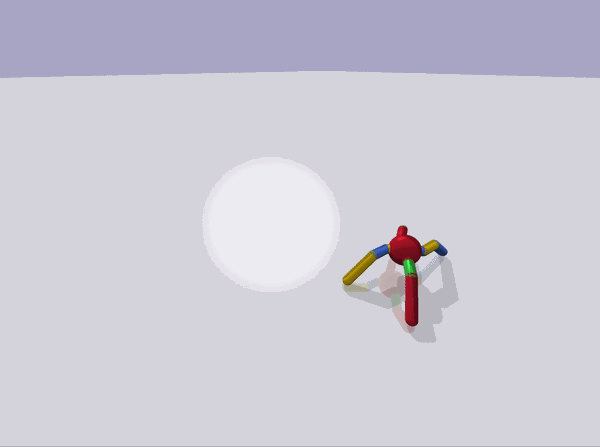
\includegraphics[scale=0.2]{../images/ant.png}}
      {\centering 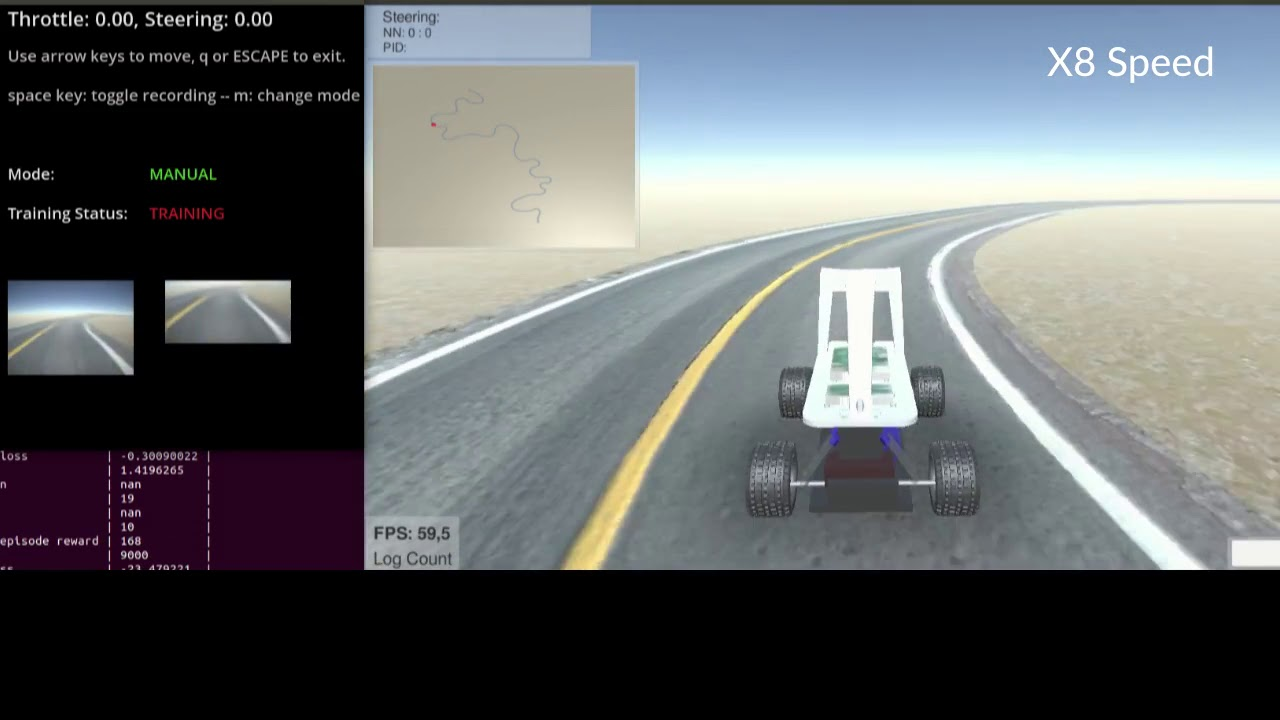
\includegraphics[scale=0.1]{../images/sac_car.jpg}}
    \end{column}

    \begin{column}{0.5\textwidth}
      {\centering 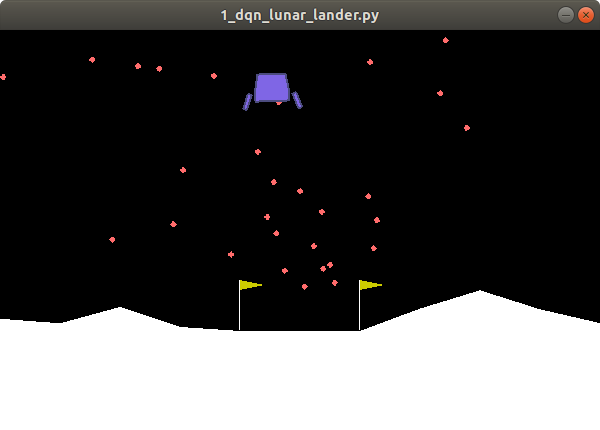
\includegraphics[scale=0.2]{../images/lunar_lander.png}}
      {\centering 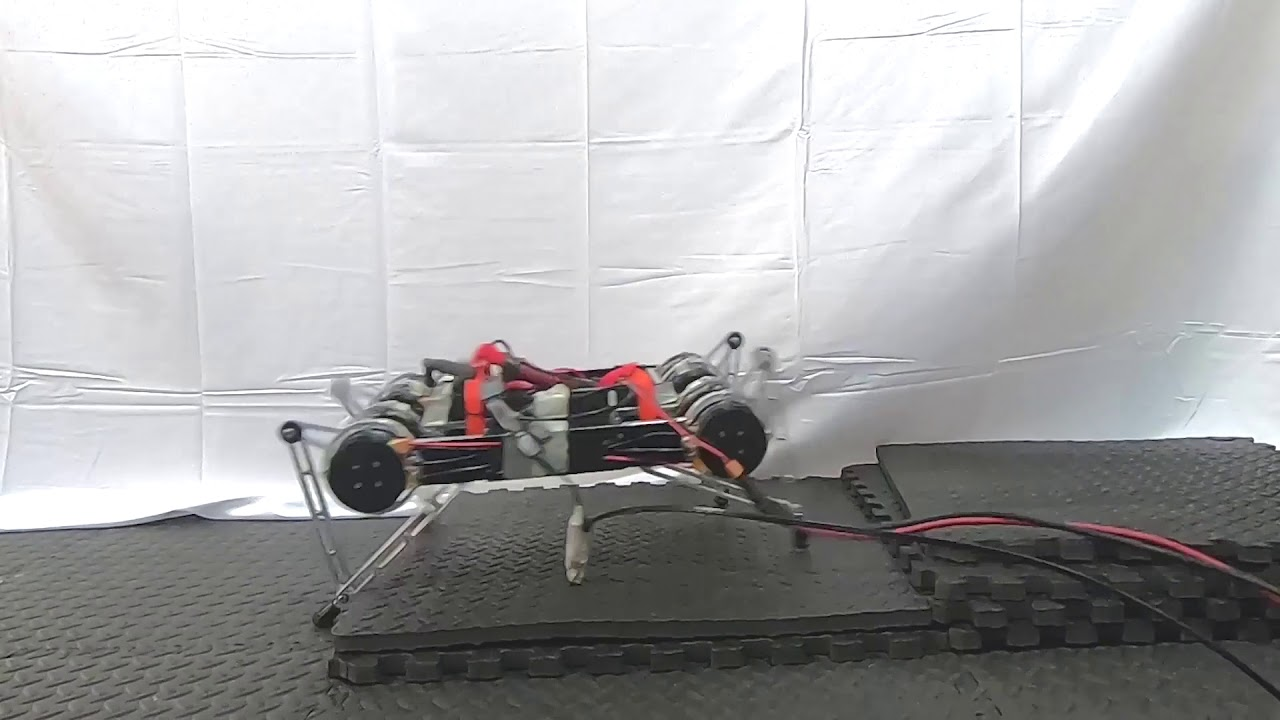
\includegraphics[scale=0.1]{../images/sac_minitaur.jpg}}
    \end{column}


  \end{columns}

\end{frame}


\begin{frame}{\bf continuous actions space}

  \begin{columns}[t]

    \begin{column}{0.5\textwidth}
      {\centering 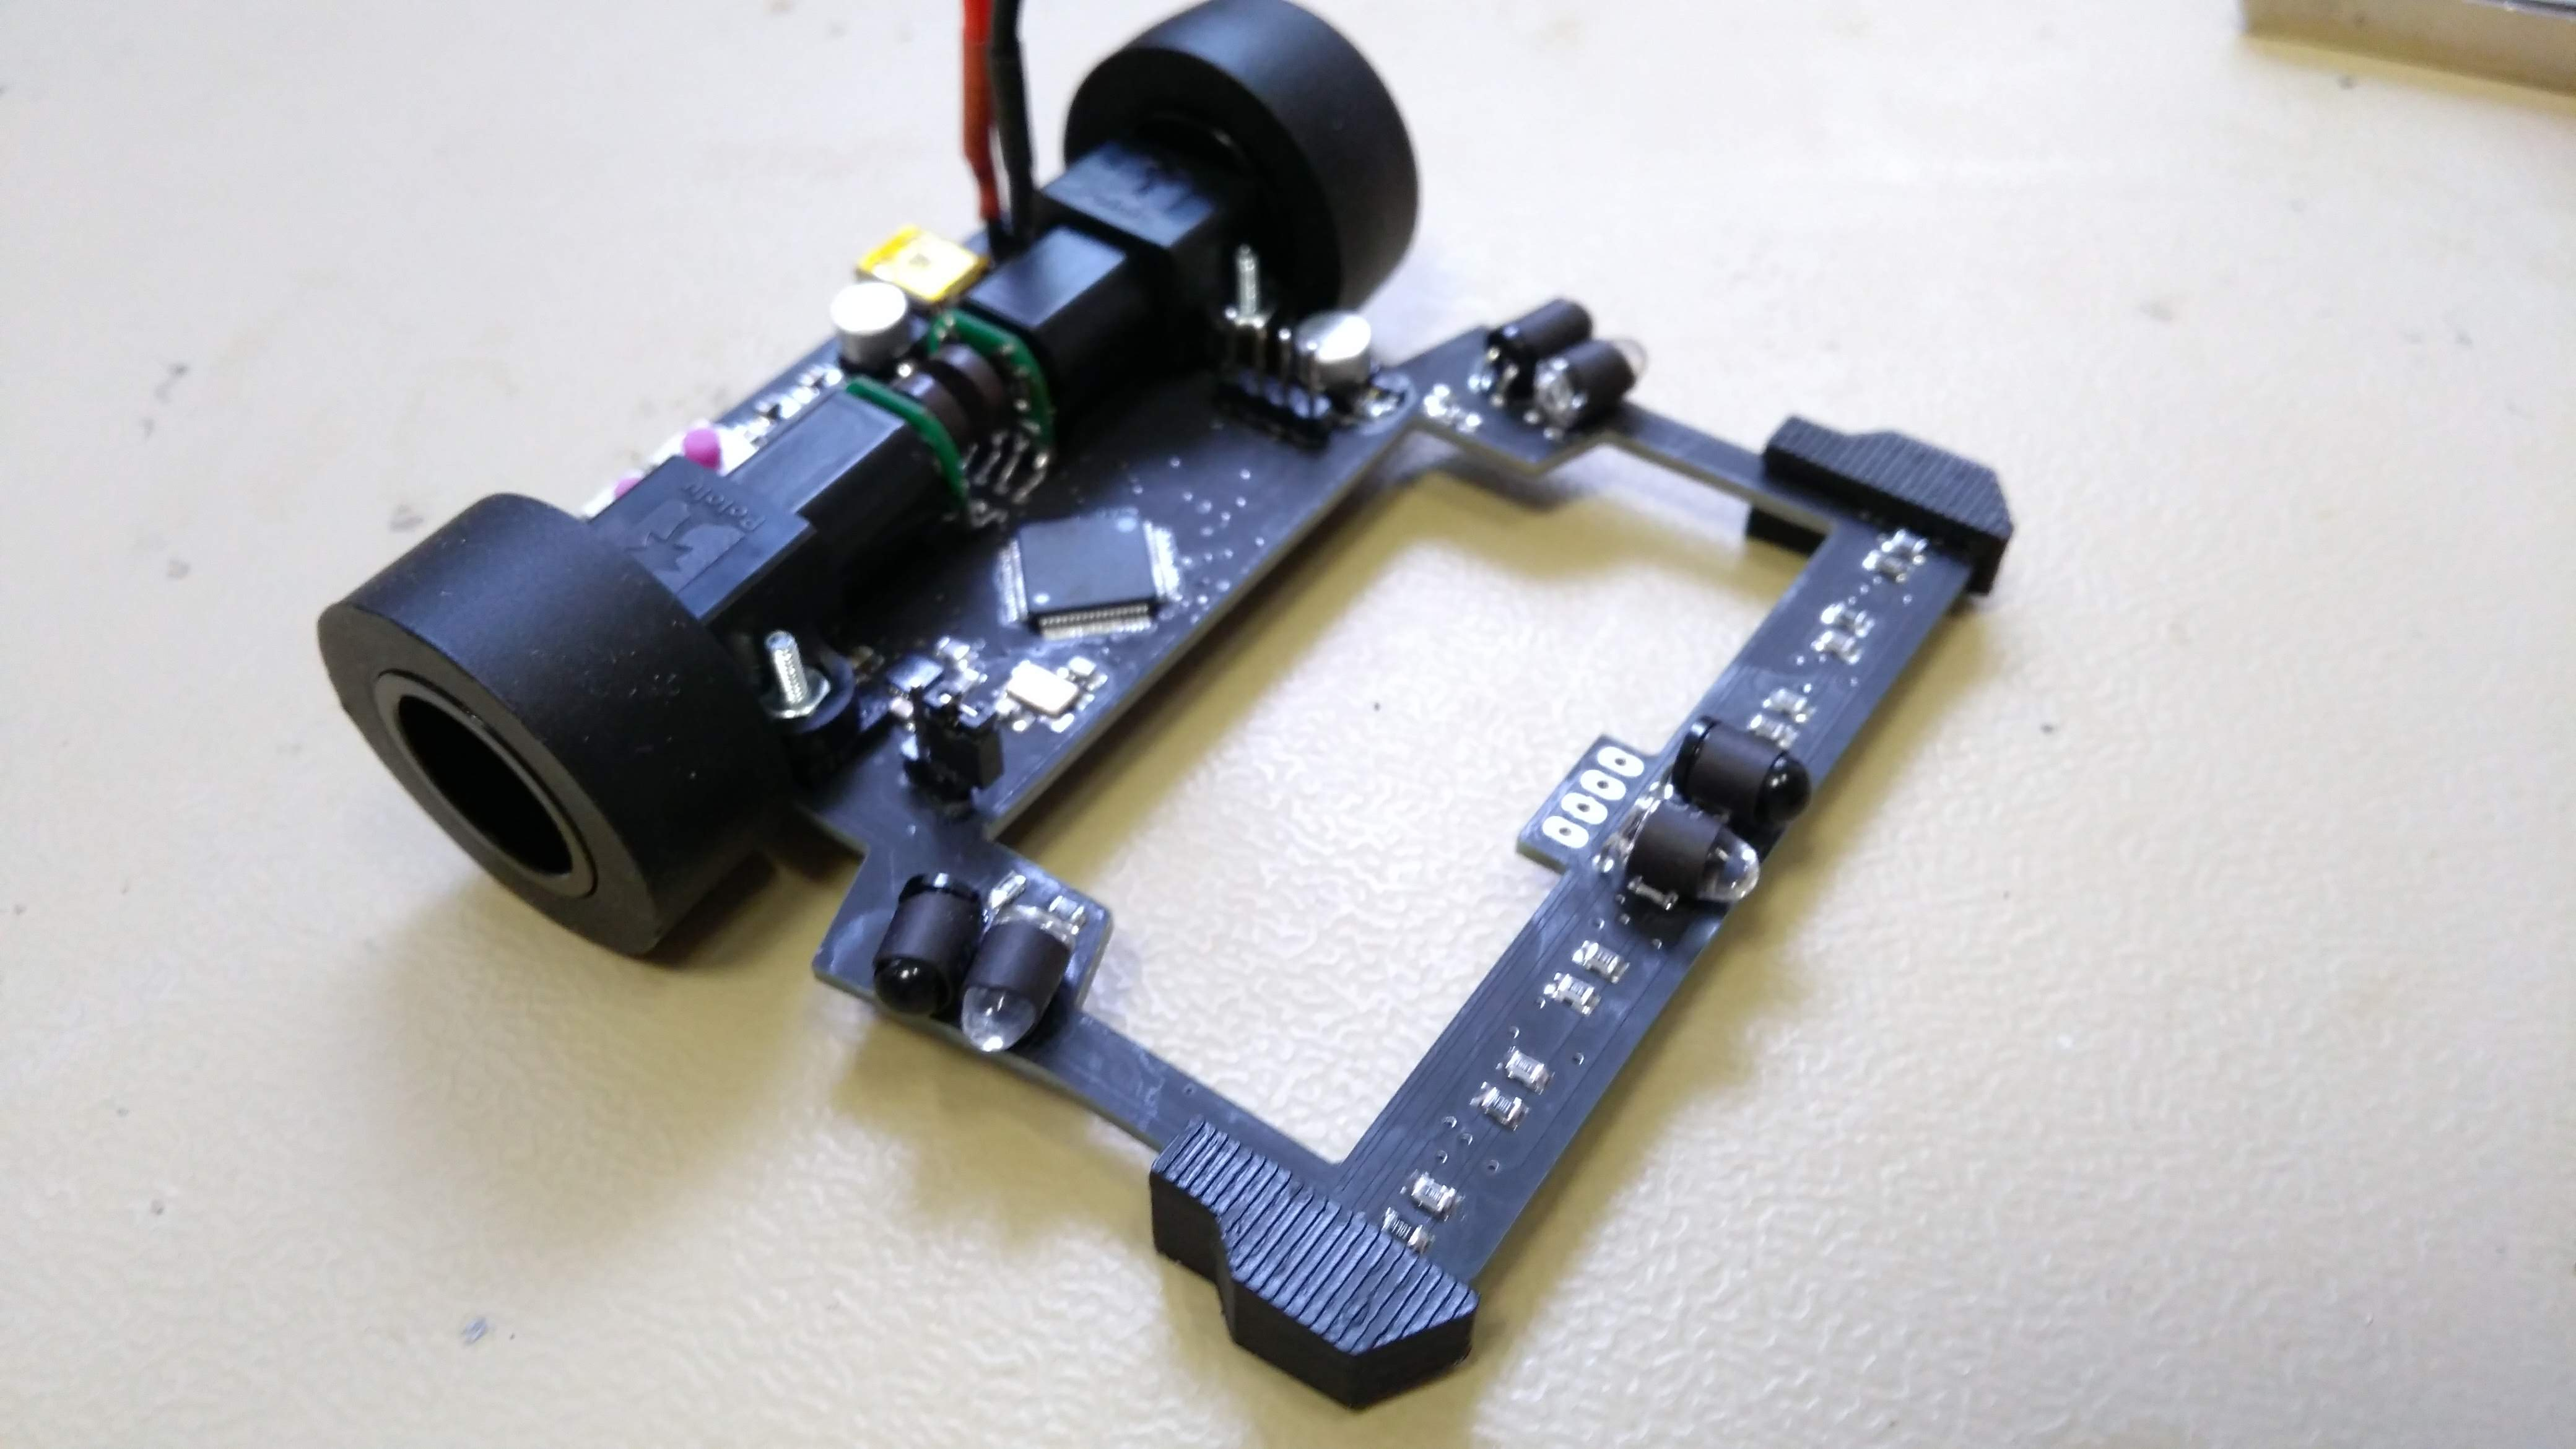
\includegraphics[scale=0.04]{../images/motoko_uprising.jpg}}
    \end{column}

    \begin{column}{0.5\textwidth}
      {\centering 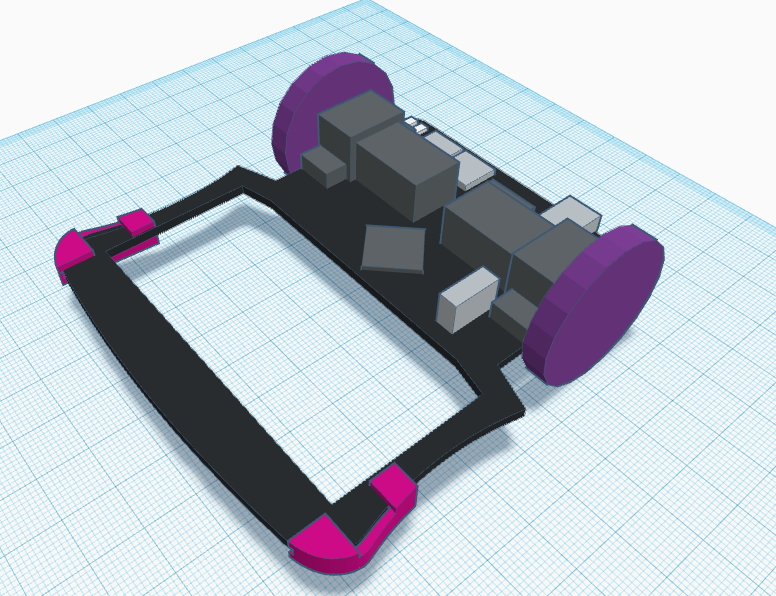
\includegraphics[scale=0.2]{../images/robot_model.png}}
    \end{column}


  \end{columns}

\end{frame}


\begin{frame}{\bf algorithms}
   \begin{itemize}
    \item discrete actions space

        \begin{itemize}
          \item Deep Q-network, DQN
          \item Dueling DQN
          \item Reinbow DQN
        \end{itemize}

    \item continuous actions space
    
        \begin{itemize}
          \item Actor Critic
          \item Advantage Actor Critic
          \item Proximal policy optimization
          \item Soft Actor critic
          \item Deep deterministc policy gradient
          \item D4PG, SDDPG
        \end{itemize}

    \item model based
    
        \begin{itemize}
          \item curiosity
          \item world models
          \item imagination agents
        \end{itemize}

  \end{itemize}

  f.e. SDDPG - sampled DDPG, based on Wasserstein loss : Optimal transport, Cédric Villani, 600+ pages

\end{frame}


\begin{frame}{\bf from DQN to DDPG}

  {\centering 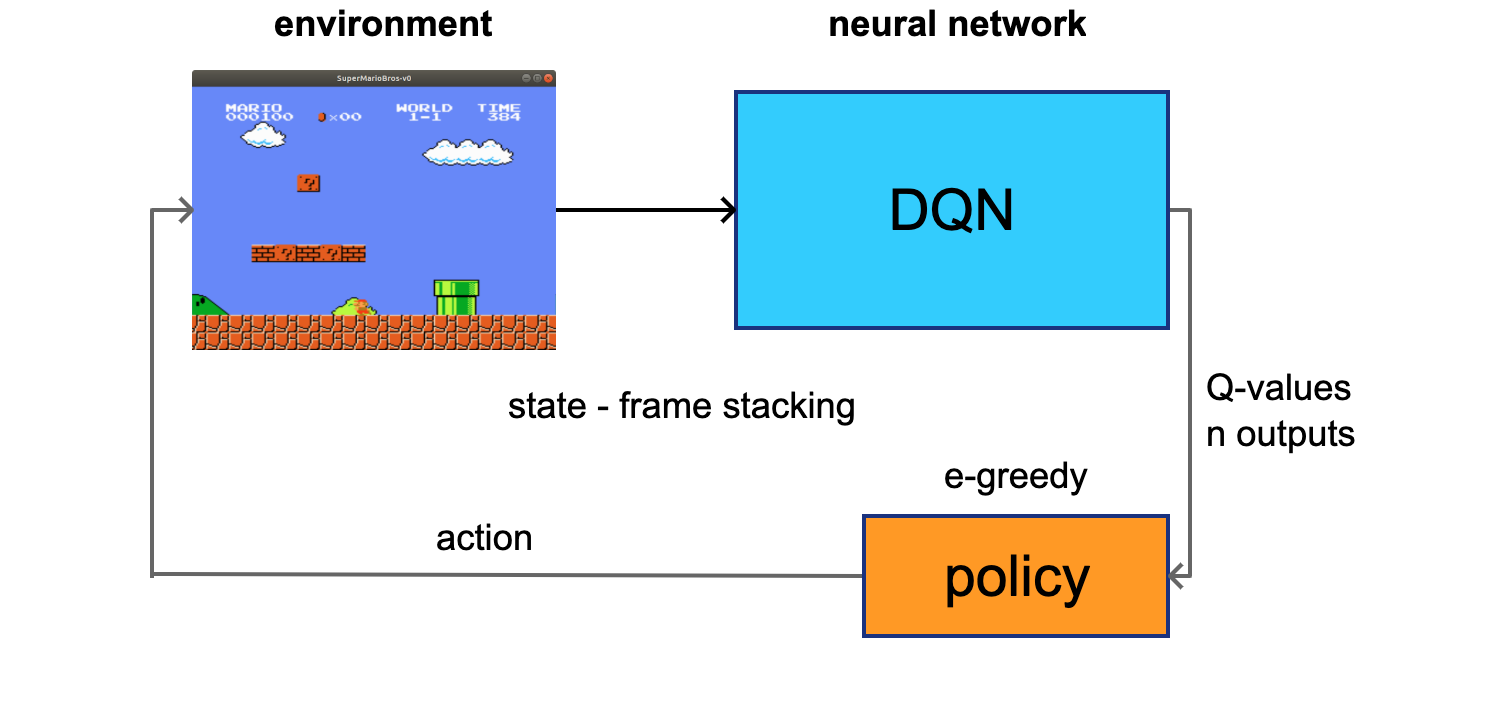
\includegraphics[scale=0.2]{../diagrams/dqn.png}}
\end{frame}

\begin{frame}{\bf from DQN to DDPG}

  {\centering 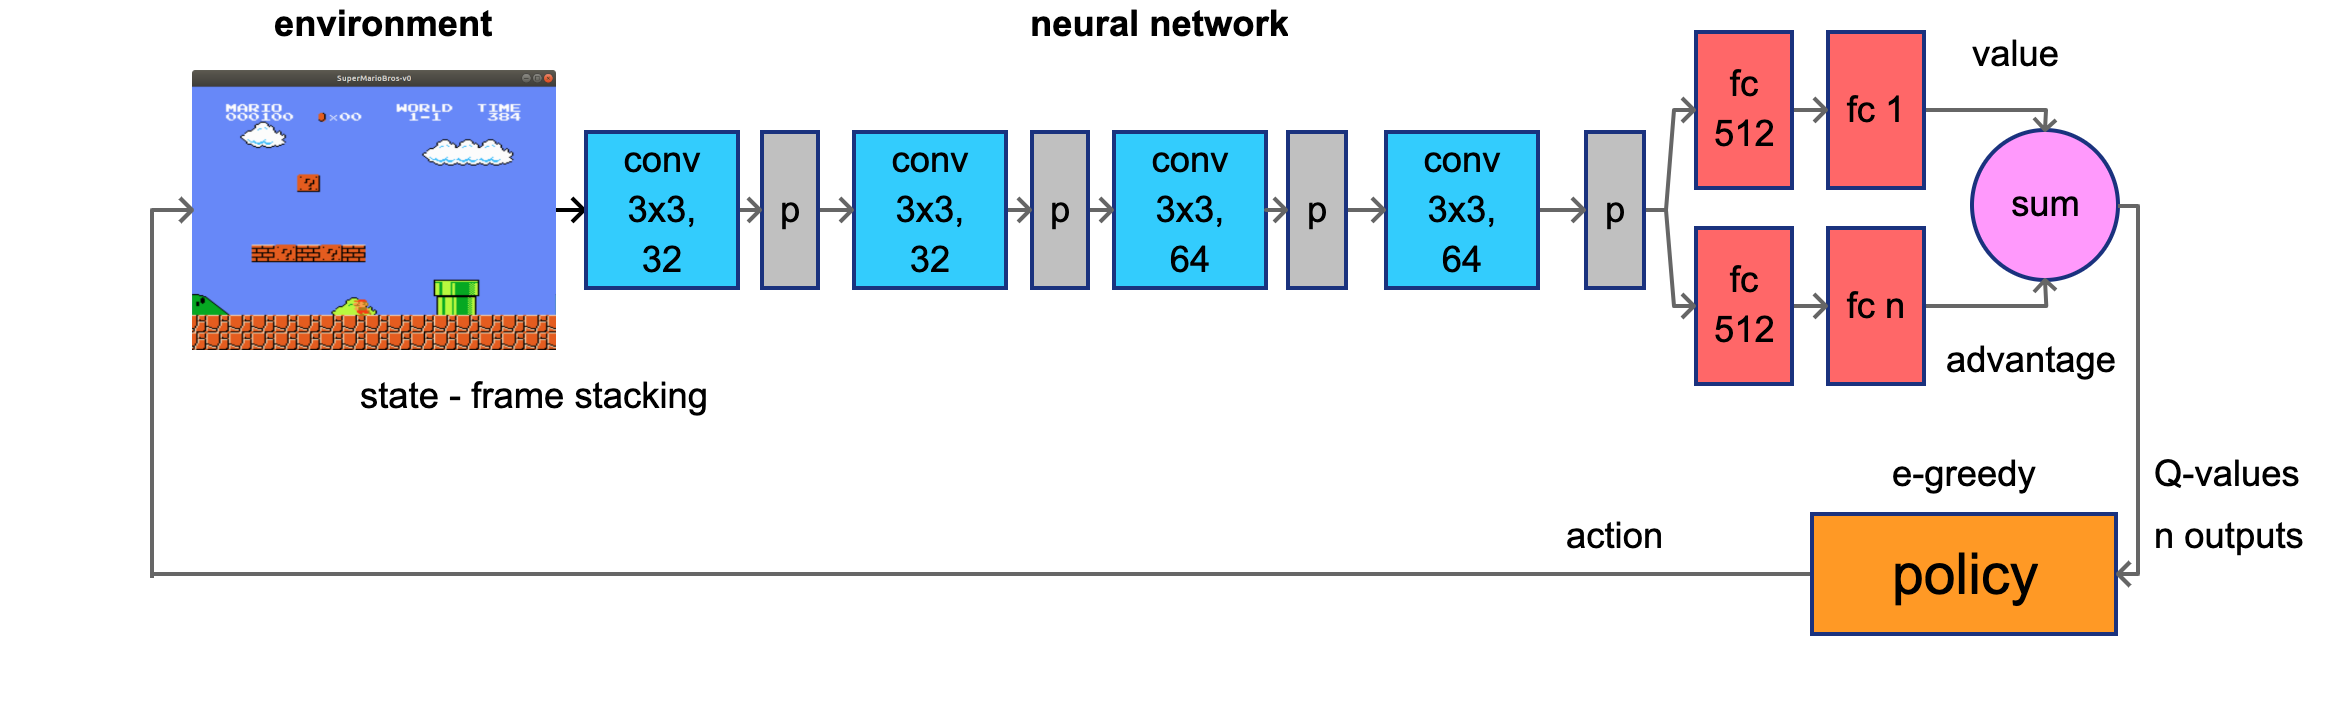
\includegraphics[scale=0.14]{../diagrams/dqndetail.png}}
\end{frame}

\begin{frame}{\bf from DQN to DDPG}

  {\centering 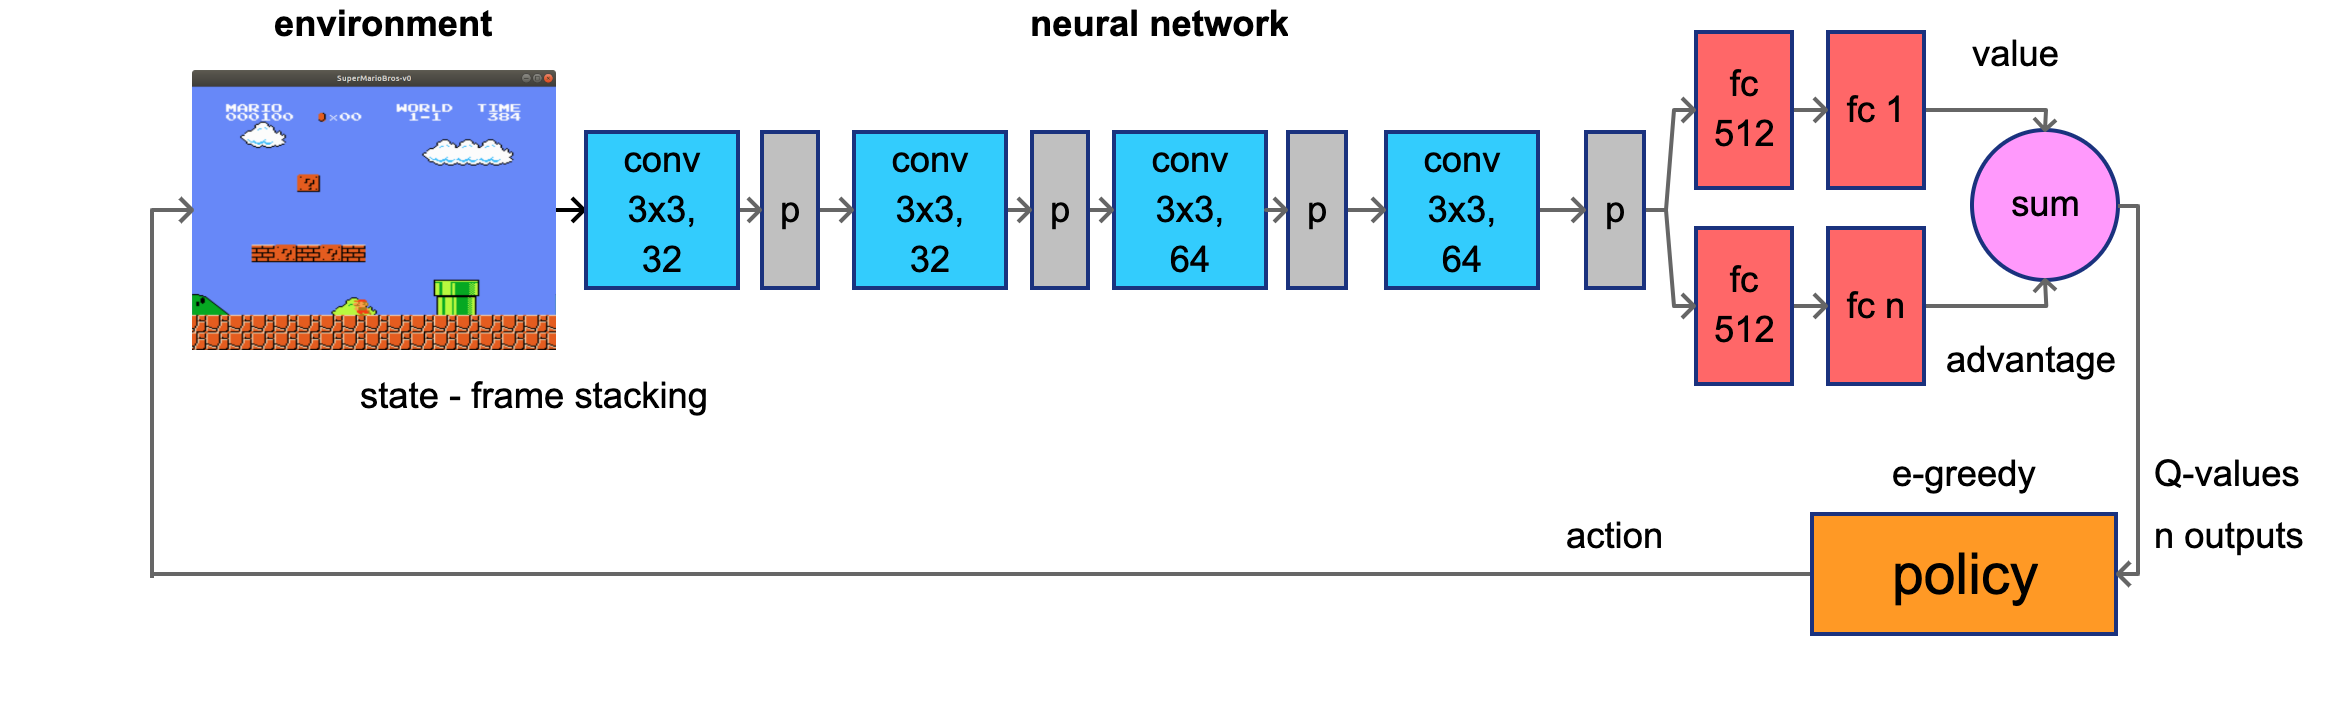
\includegraphics[scale=0.14]{../diagrams/dqndetail.png}}

    \begin{align*}
      \mathcal{L(\theta)} = \left( R + \gamma \max \limits_{a'} Q(s', a'; \theta^-) - Q(s, a; \theta)  \right)^2
    \end{align*}
\end{frame}

\begin{frame}{\bf from DQN to DDPG}

  {\centering 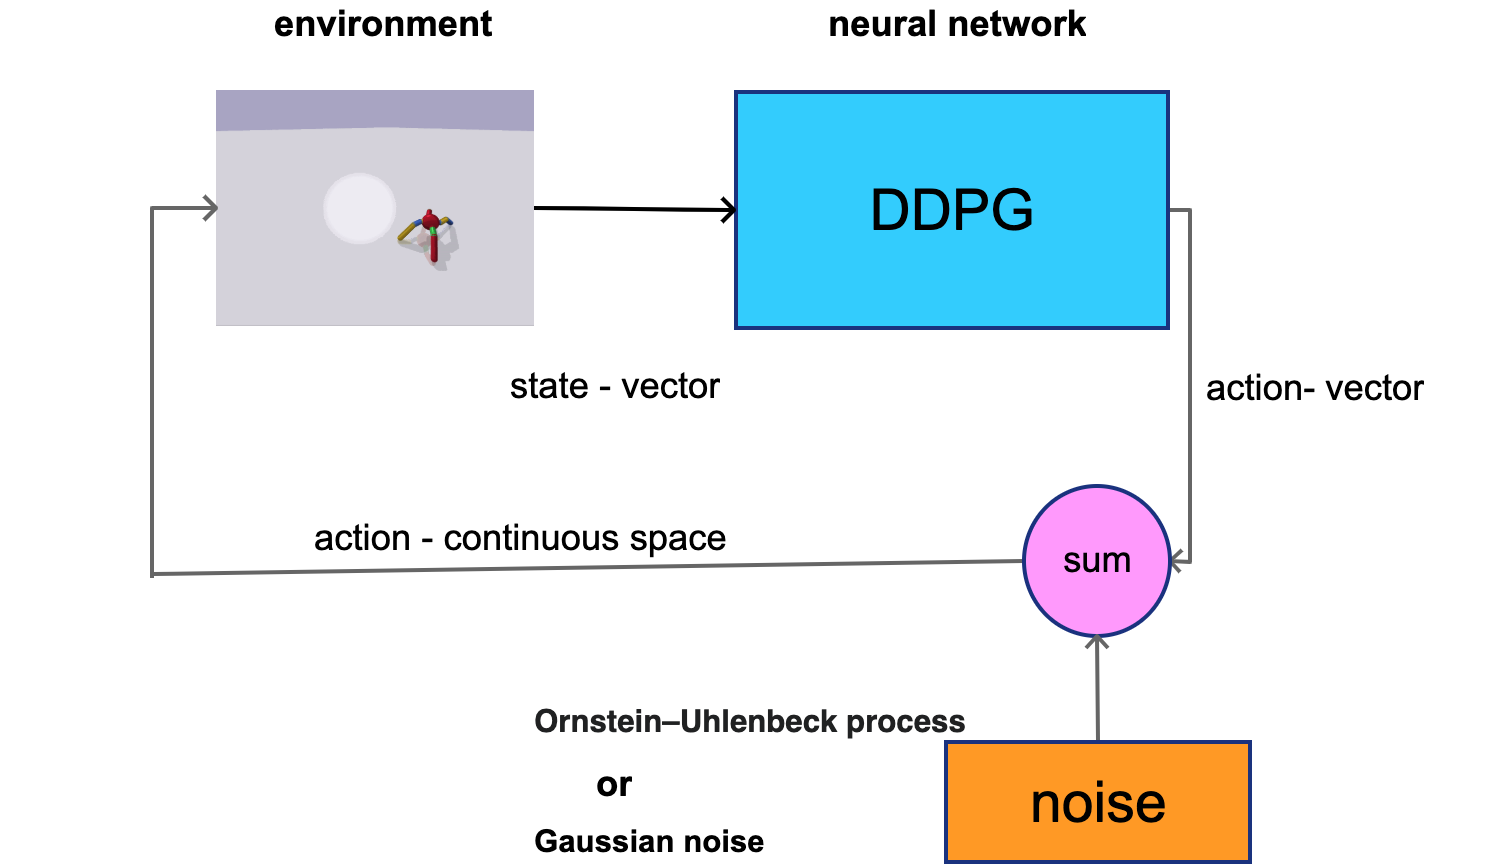
\includegraphics[scale=0.2]{../diagrams/ddpg.png}}
\end{frame}

\begin{frame}{\bf from DQN to DDPG}

  {\centering 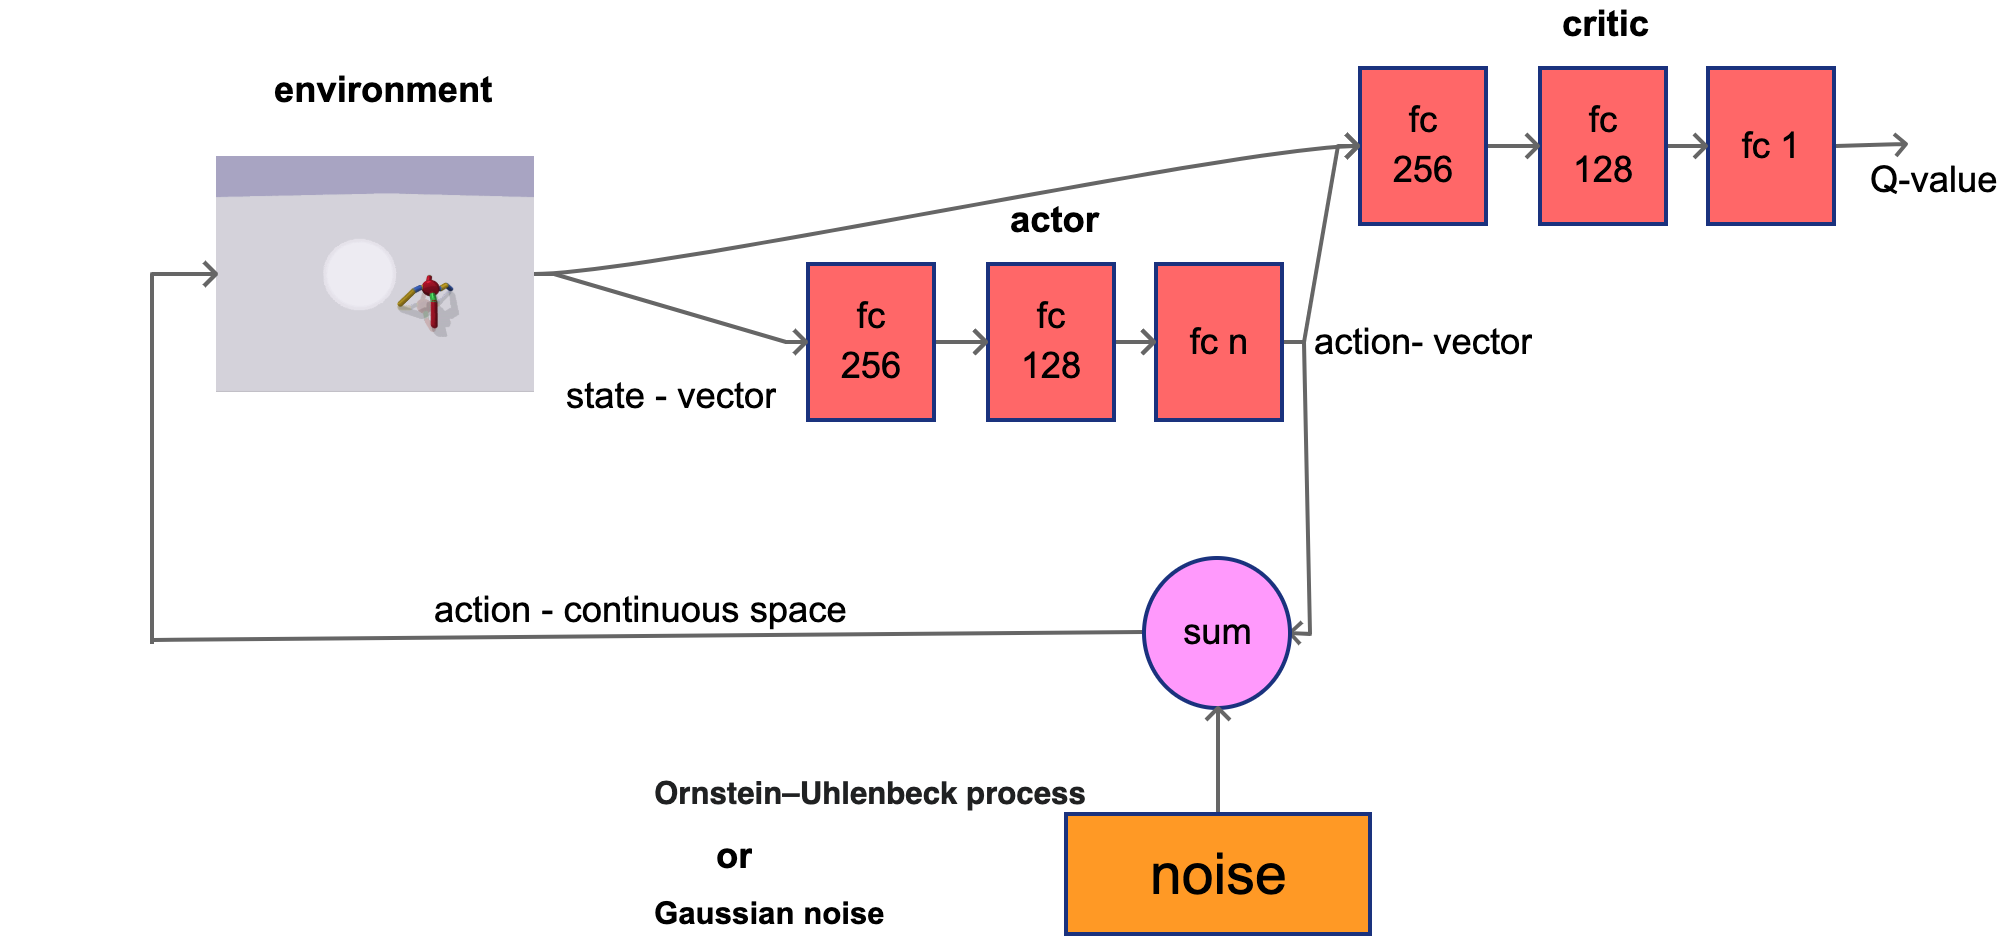
\includegraphics[scale=0.16]{../diagrams/ddpgdetail.png}}
\end{frame}

\begin{frame}{\bf from DQN to DDPG}

  {\centering 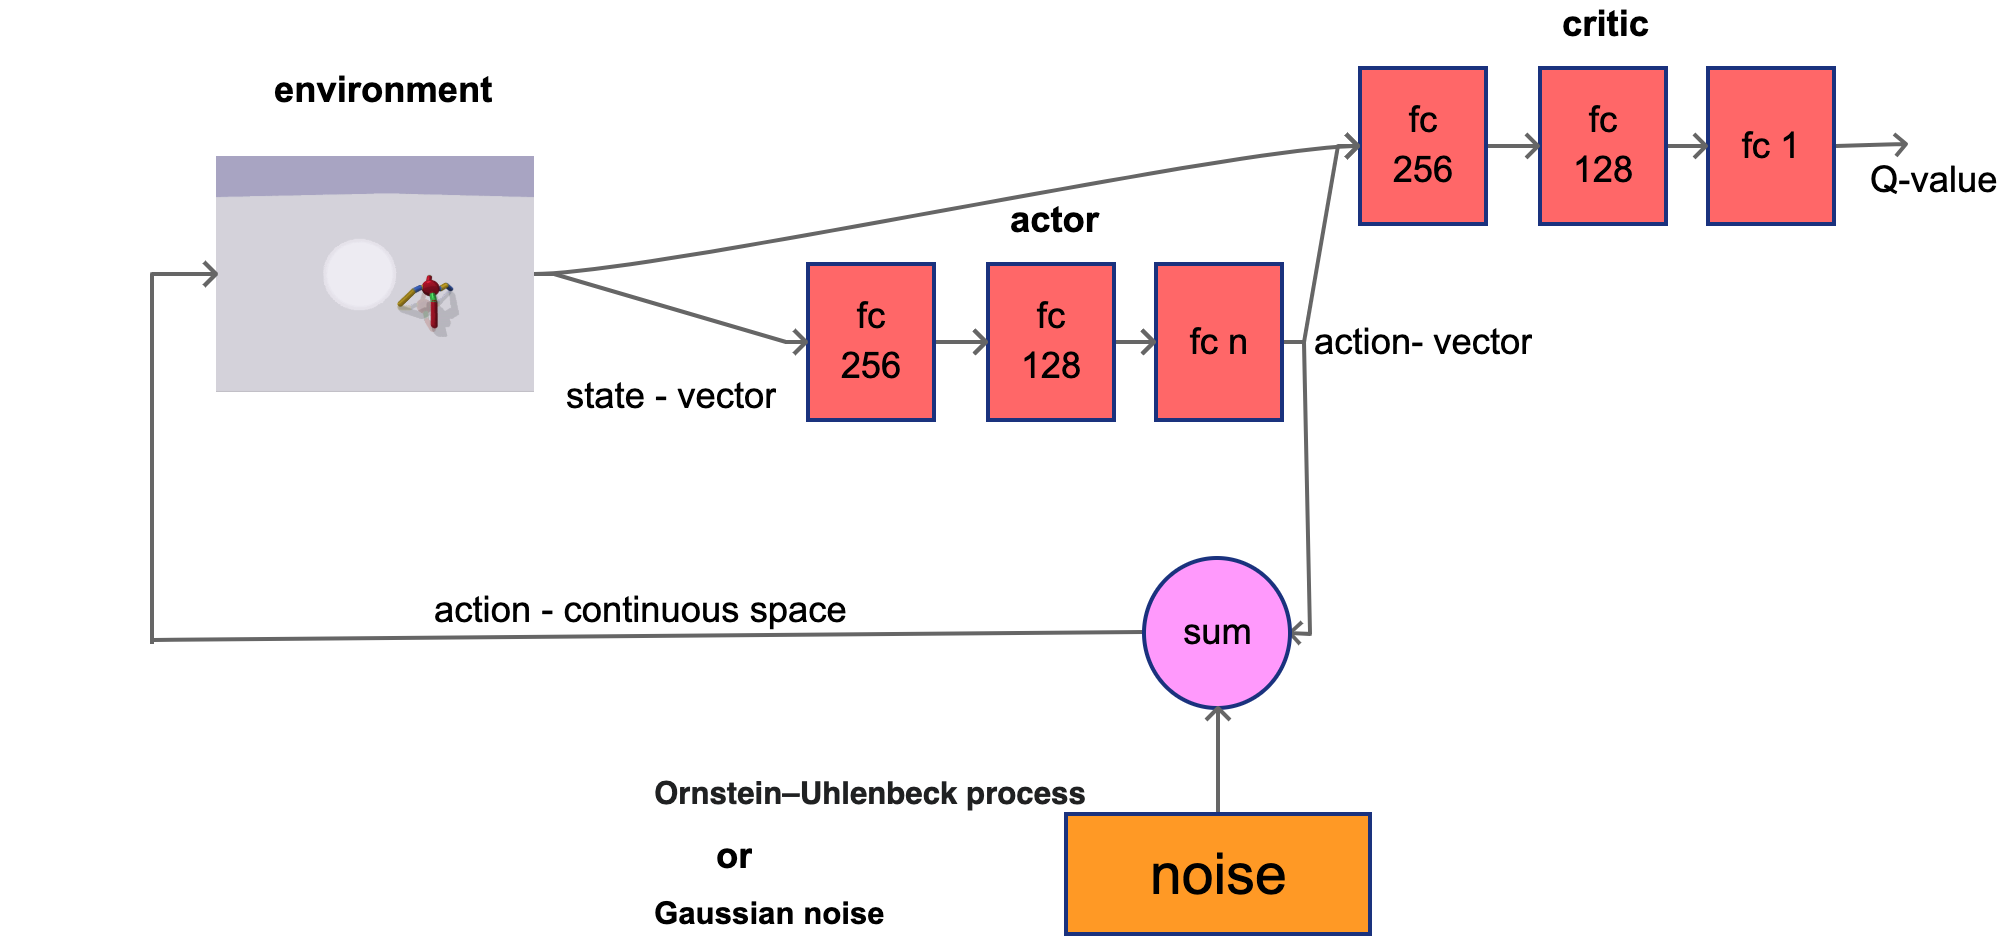
\includegraphics[scale=0.16]{../diagrams/ddpgdetail.png}}

    critic loss:
    \begin{align*}
      \mathcal{L}_c(\theta) = \left( R + \gamma Q(s', a'; \theta^-, \phi^- ) - Q(s, a; \theta, \phi )  \right)^2
    \end{align*}

    actor loss :
    \begin{align*}
      \mathcal{L}_a(\phi) = -Q(s, a; \theta, \phi)
    \end{align*}
\end{frame}



\begin{frame}{\bf reparametrization trick}

   \begin{columns}[t]

    \begin{column}{0.5\textwidth}
      non-differentiable \\
      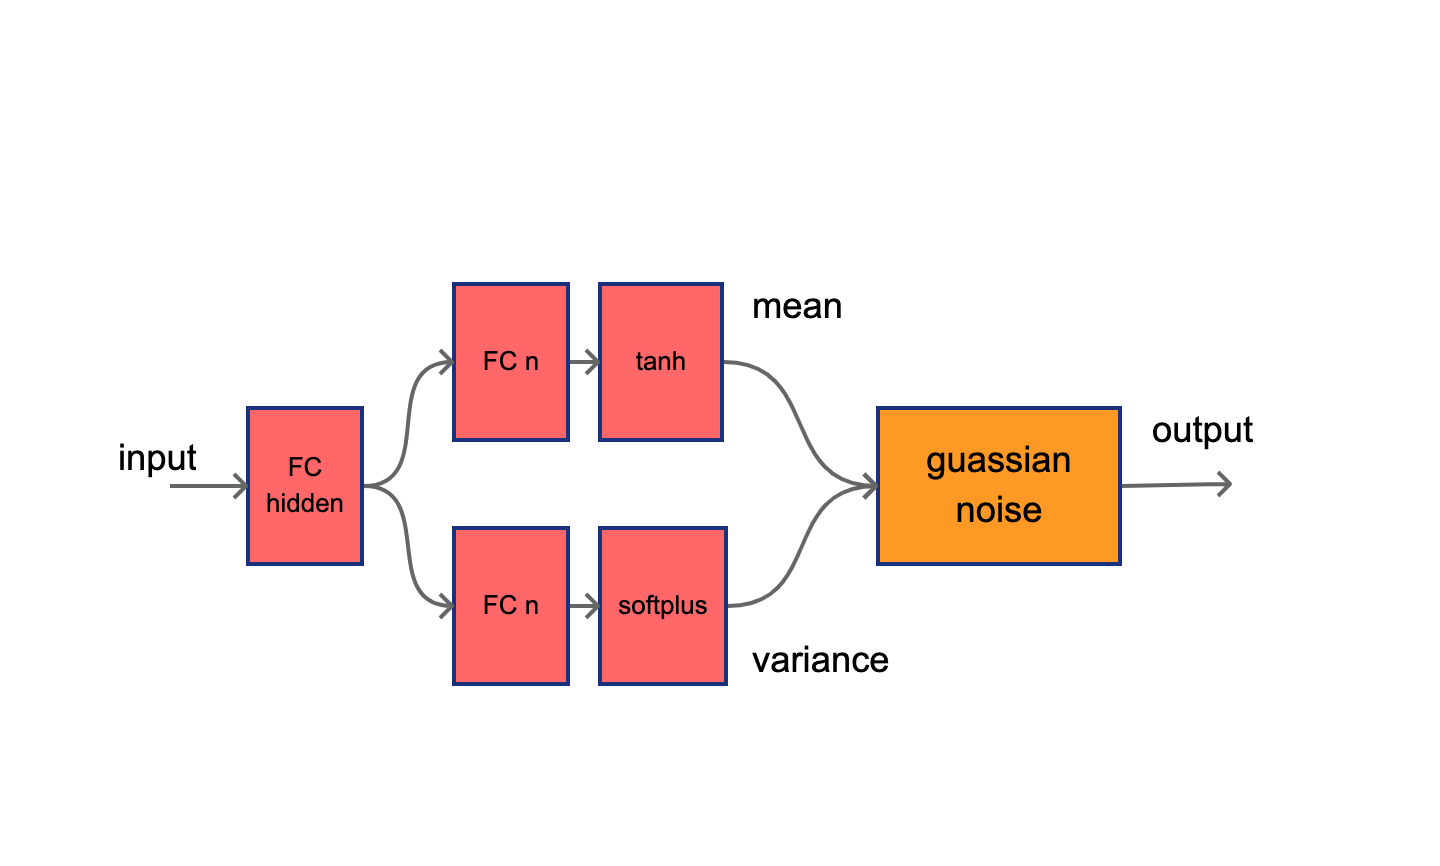
\includegraphics[scale=0.11]{../diagrams/reparametrizationtrick0.png}

      \begin{align*}
        \frac{\partial {y}}{\partial {f_{noise}(x)}} = \frac{\partial {y}}{\partial {f_{noise}}}\frac{\partial {f_{noise}}}{\partial {x}}
      \end{align*}
    \end{column}

    \begin{column}{0.5\textwidth}
      differentiable \\
      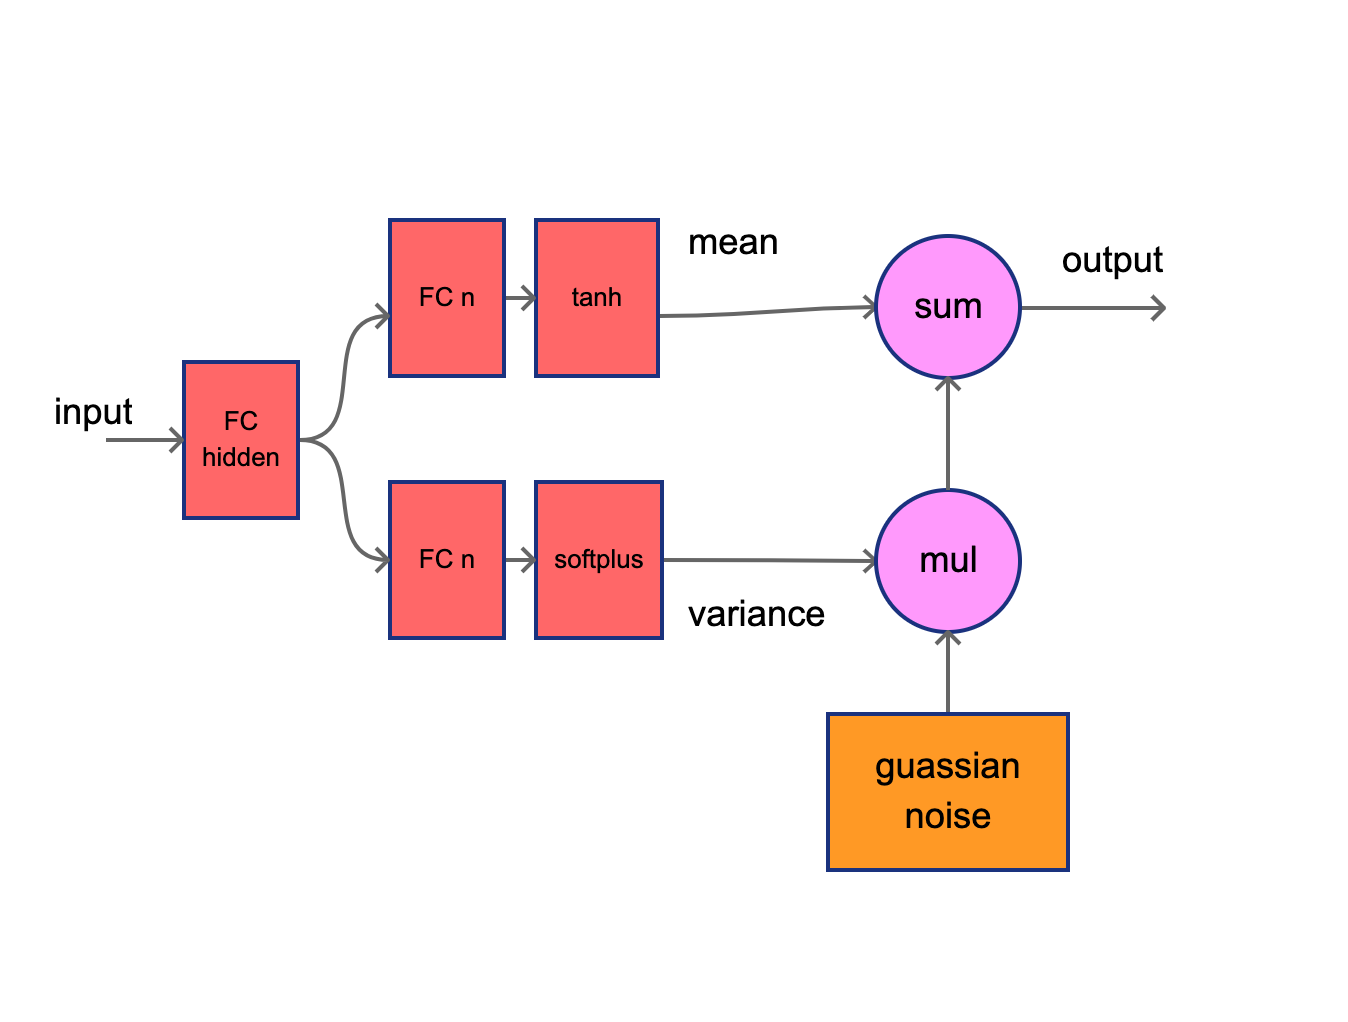
\includegraphics[scale=0.11]{../diagrams/reparametrizationtrick1.png}
    \end{column}

  \end{columns}

\end{frame}




\begin{frame}{\bf wise Wizard's DDPG spell chart}
  \begin{itemize}
    \item {\bf \color{red} neurons count} on 1st layer = 10x  state vector size
    \item {\bf \color{red} neurons count} on 2nd layer = 0.5x neurons on 1st layer
    \item {\bf \color{red} weight init} for hidden layers : use Xavier
    \item {\bf \color{red} weight init} actor output  : use uniform $\langle -0.3, 0.3 \rangle$
    \item {\bf \color{red} weight init} critic output : use uniform $\langle -0.003, 0.003 \rangle$
    \item {\bf \color{red} gaussian noise} : linear decay variance, from 1 to 0.3, for 1M steps 
    \item use {\bf \color{red} soft} target network update, $\tau = 0.001$
    \item actor learning rate $\eta_a = 0.0001$
    \item critic learning rate $\eta_c = 0.0002$
  \end{itemize}
\end{frame}


\begin{frame}{\bf DDPG critic}

  {\centering 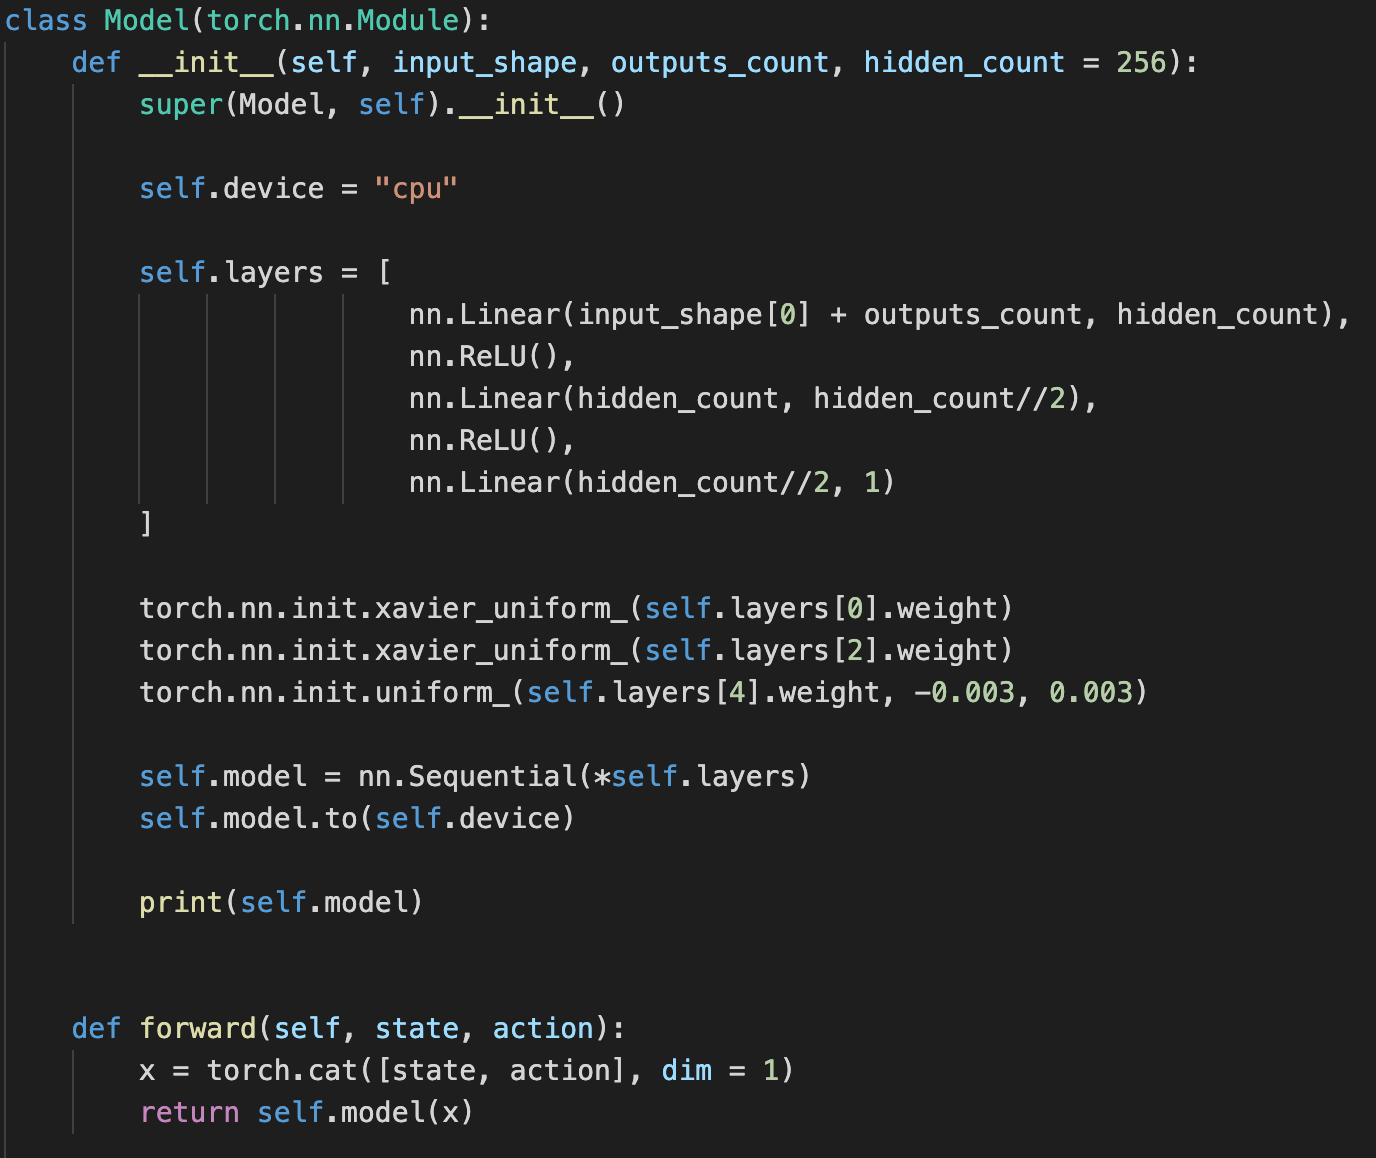
\includegraphics[scale=0.4]{../images/ddpg_critic.png}}
\end{frame}

\begin{frame}{\bf DDPG actor}

  {\centering 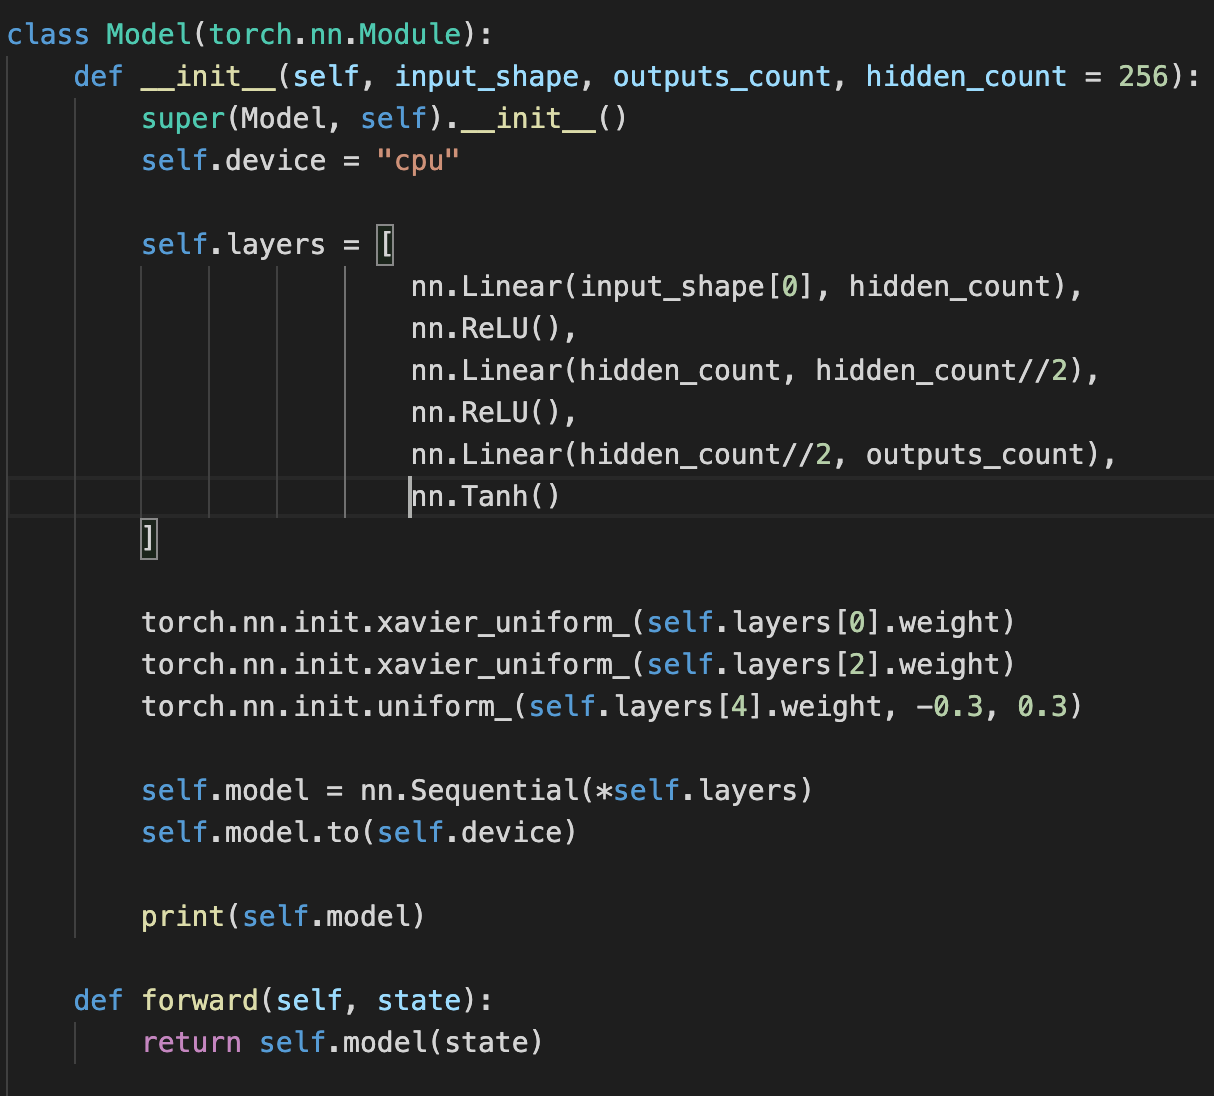
\includegraphics[scale=0.4]{../images/ddpg_actor.png}}
\end{frame}


\begin{frame}{\bf wise Wizard's magic staff}

  \begin{columns}

    \begin{column}{0.5\textwidth}
      \begin{itemize}
        \item fully connected nets (robotic envs) {\bf \color{red} train on CPU} - AMD Ryzen
        \item convolutional nets (visual inputs envs) {\bf \color{red} train on GPU} - NVIDIA GTX1080+
        \item use fast CPU - envs are slow
        \item 32GB of RAM is enough
        \item for small visual envs (Atari, DOOM, Nec) - GTX1080ti
      \end{itemize}
    \end{column}

    \begin{column}{0.5\textwidth}
      {\centering 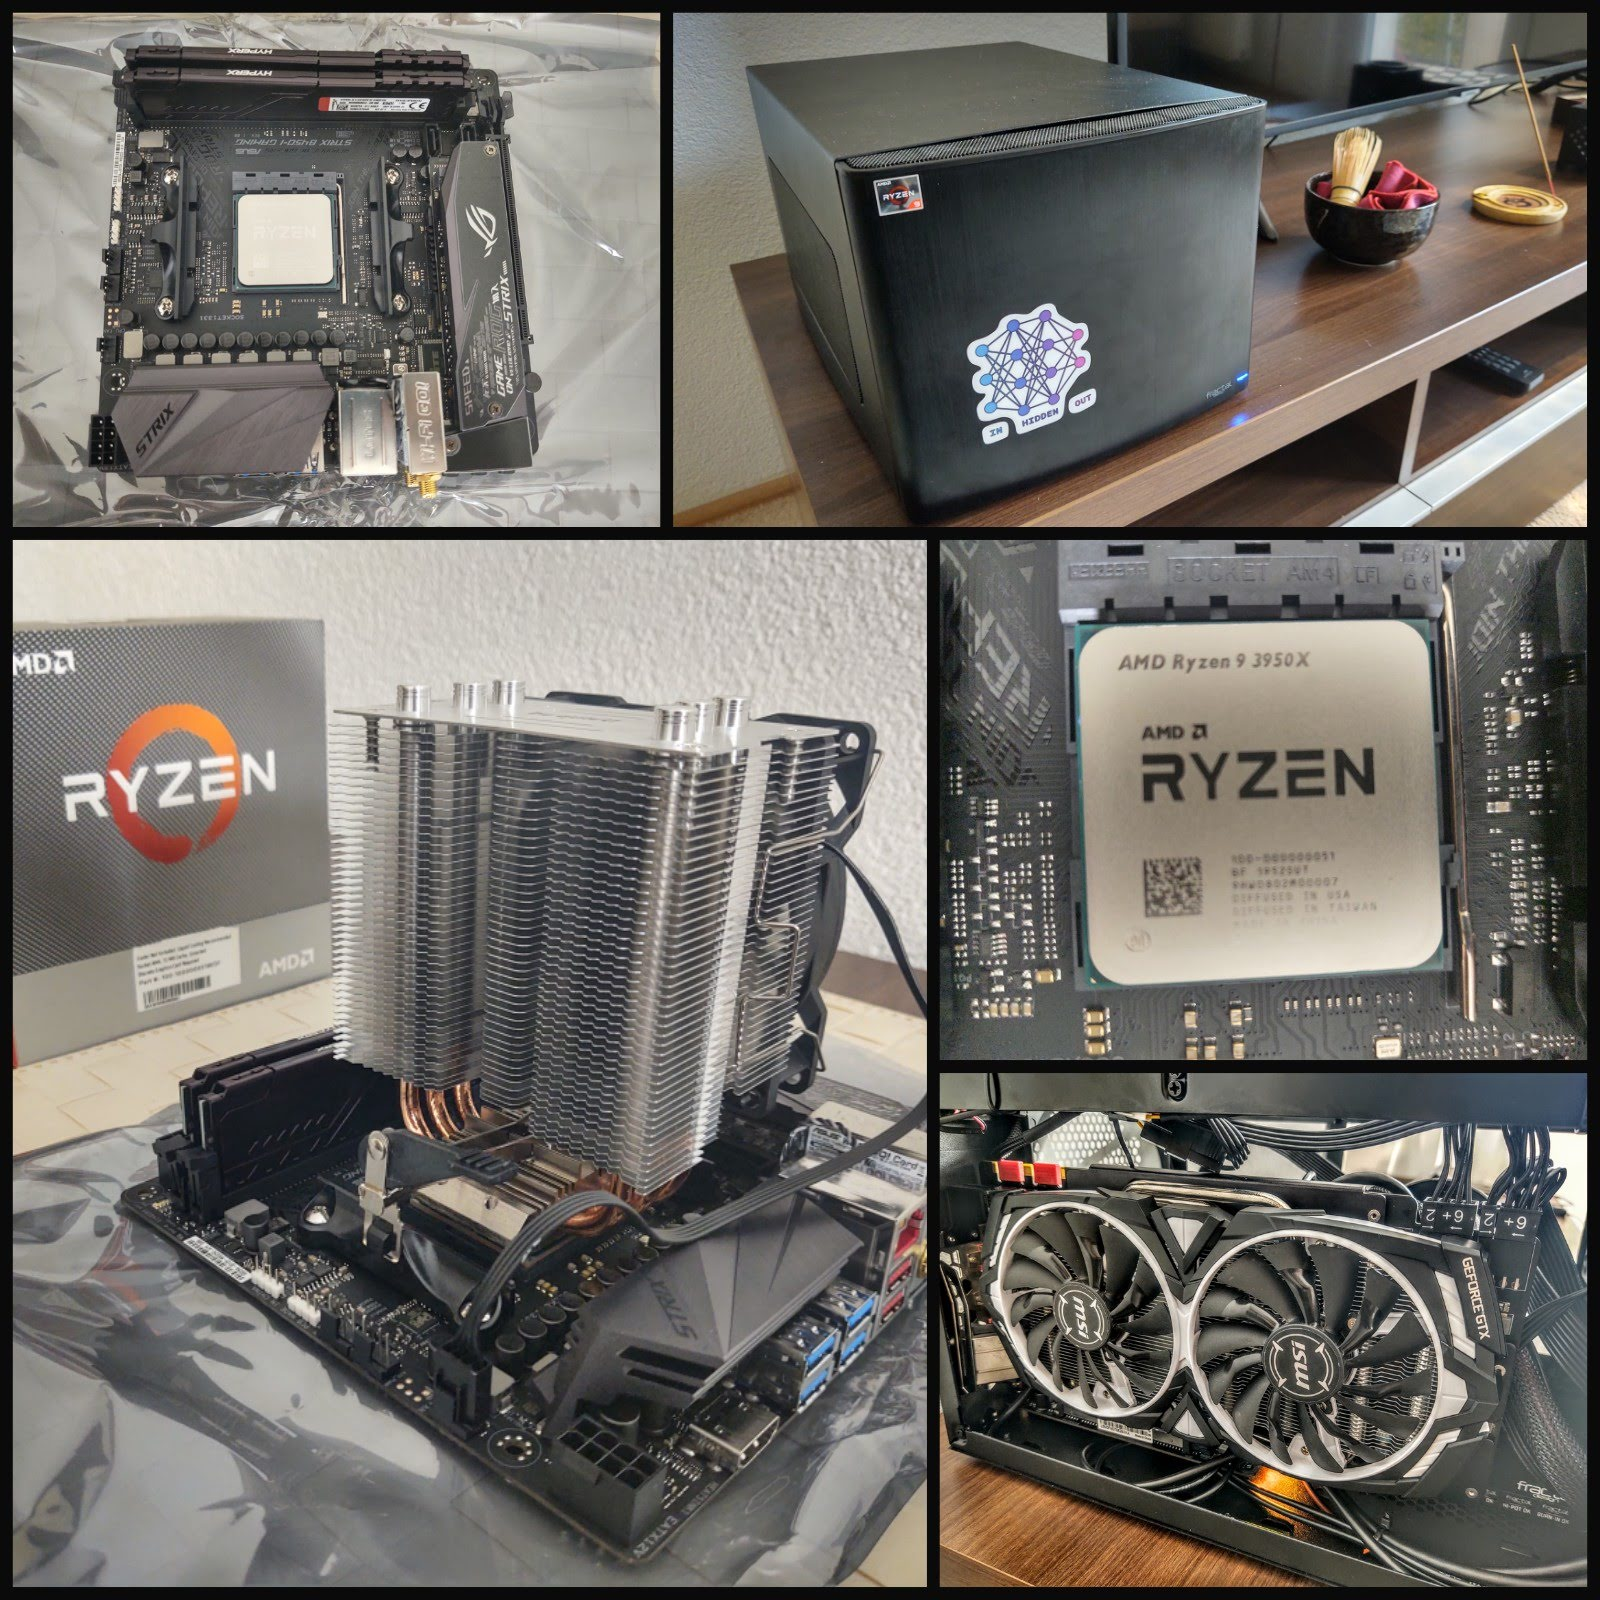
\includegraphics[scale=0.1]{../images/computer.jpg}}
    \end{column}

  \end{columns}


\end{frame}

\begin{frame}{\bf model based RL}

  {\centering 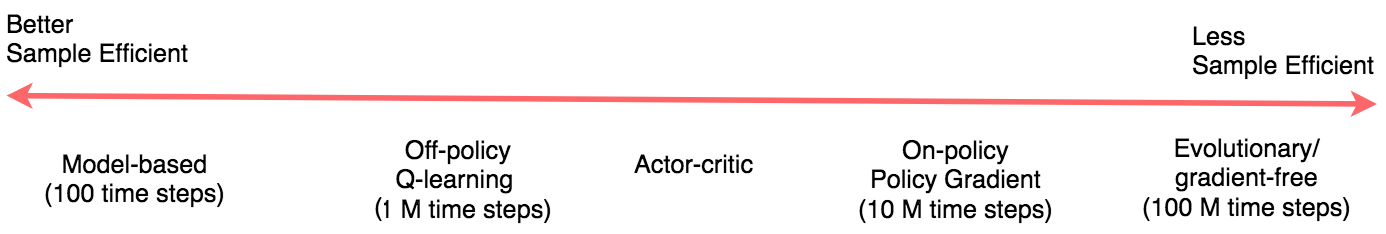
\includegraphics[scale=0.22]{../images/samples.png}}

  \begin{itemize}
    \item curiosity
    \item world models
    \item imagination
  \end{itemize}

\end{frame}

\begin{frame}{\bf curiosity in RL}

  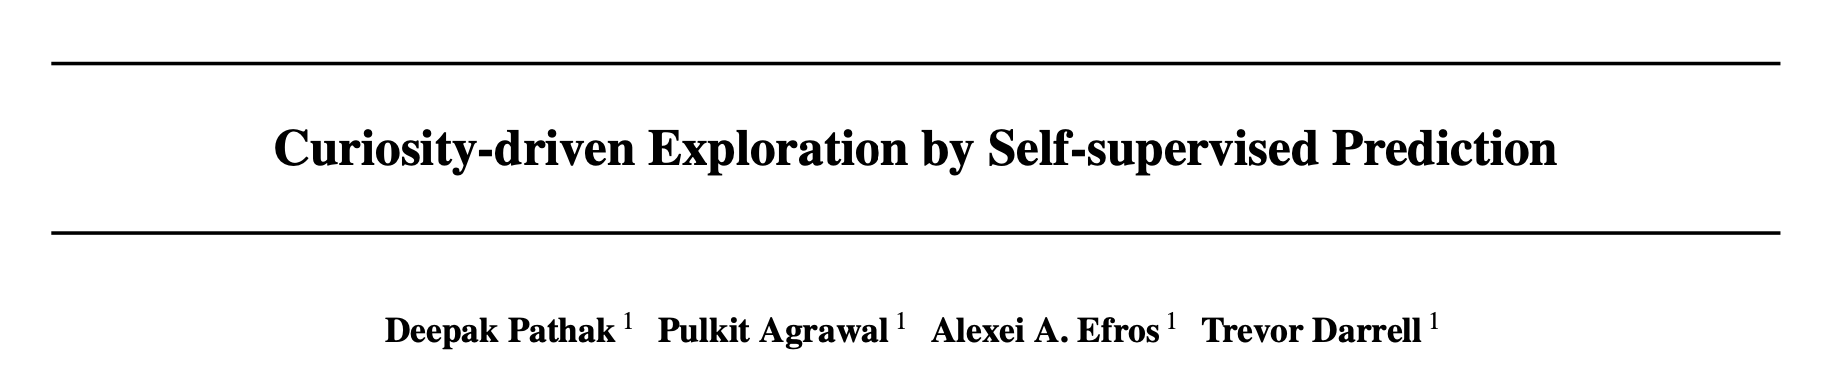
\includegraphics[scale=0.2]{../images/paper_curiosity_0.png}


  \begin{columns}

    \begin{column}{0.5\textwidth}
      \begin{itemize}
        \item Curiosity-driven Exploration by Self-supervised Prediction, 2017, Deepak Pathak
        \item old idea : adaptive controll (dynamic system identification, adaptive filtering)
        \item {\bf \color{red} main idea } : curiosity = squared model prediction error
      \end{itemize}
    \end{column}

    \begin{column}{0.5\textwidth}
      {\centering 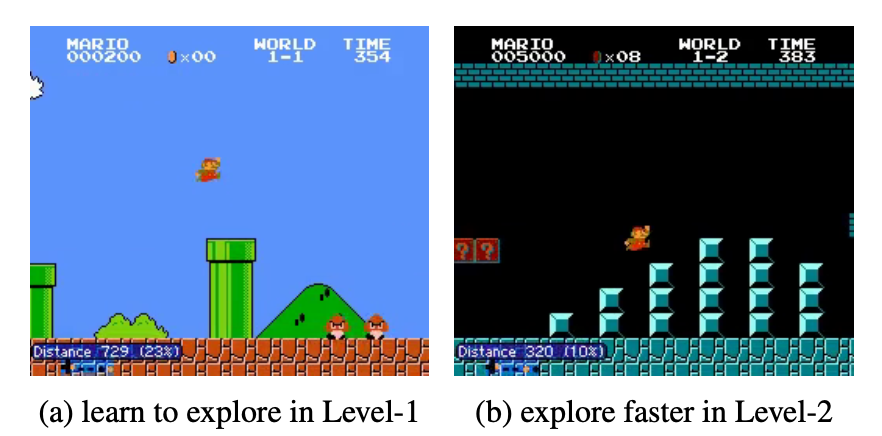
\includegraphics[scale=0.4]{../images/paper_curiosity_1.png}}
    \end{column}

  \end{columns}
\end{frame}


\begin{frame}{\bf curiosity in RL}

  {\centering 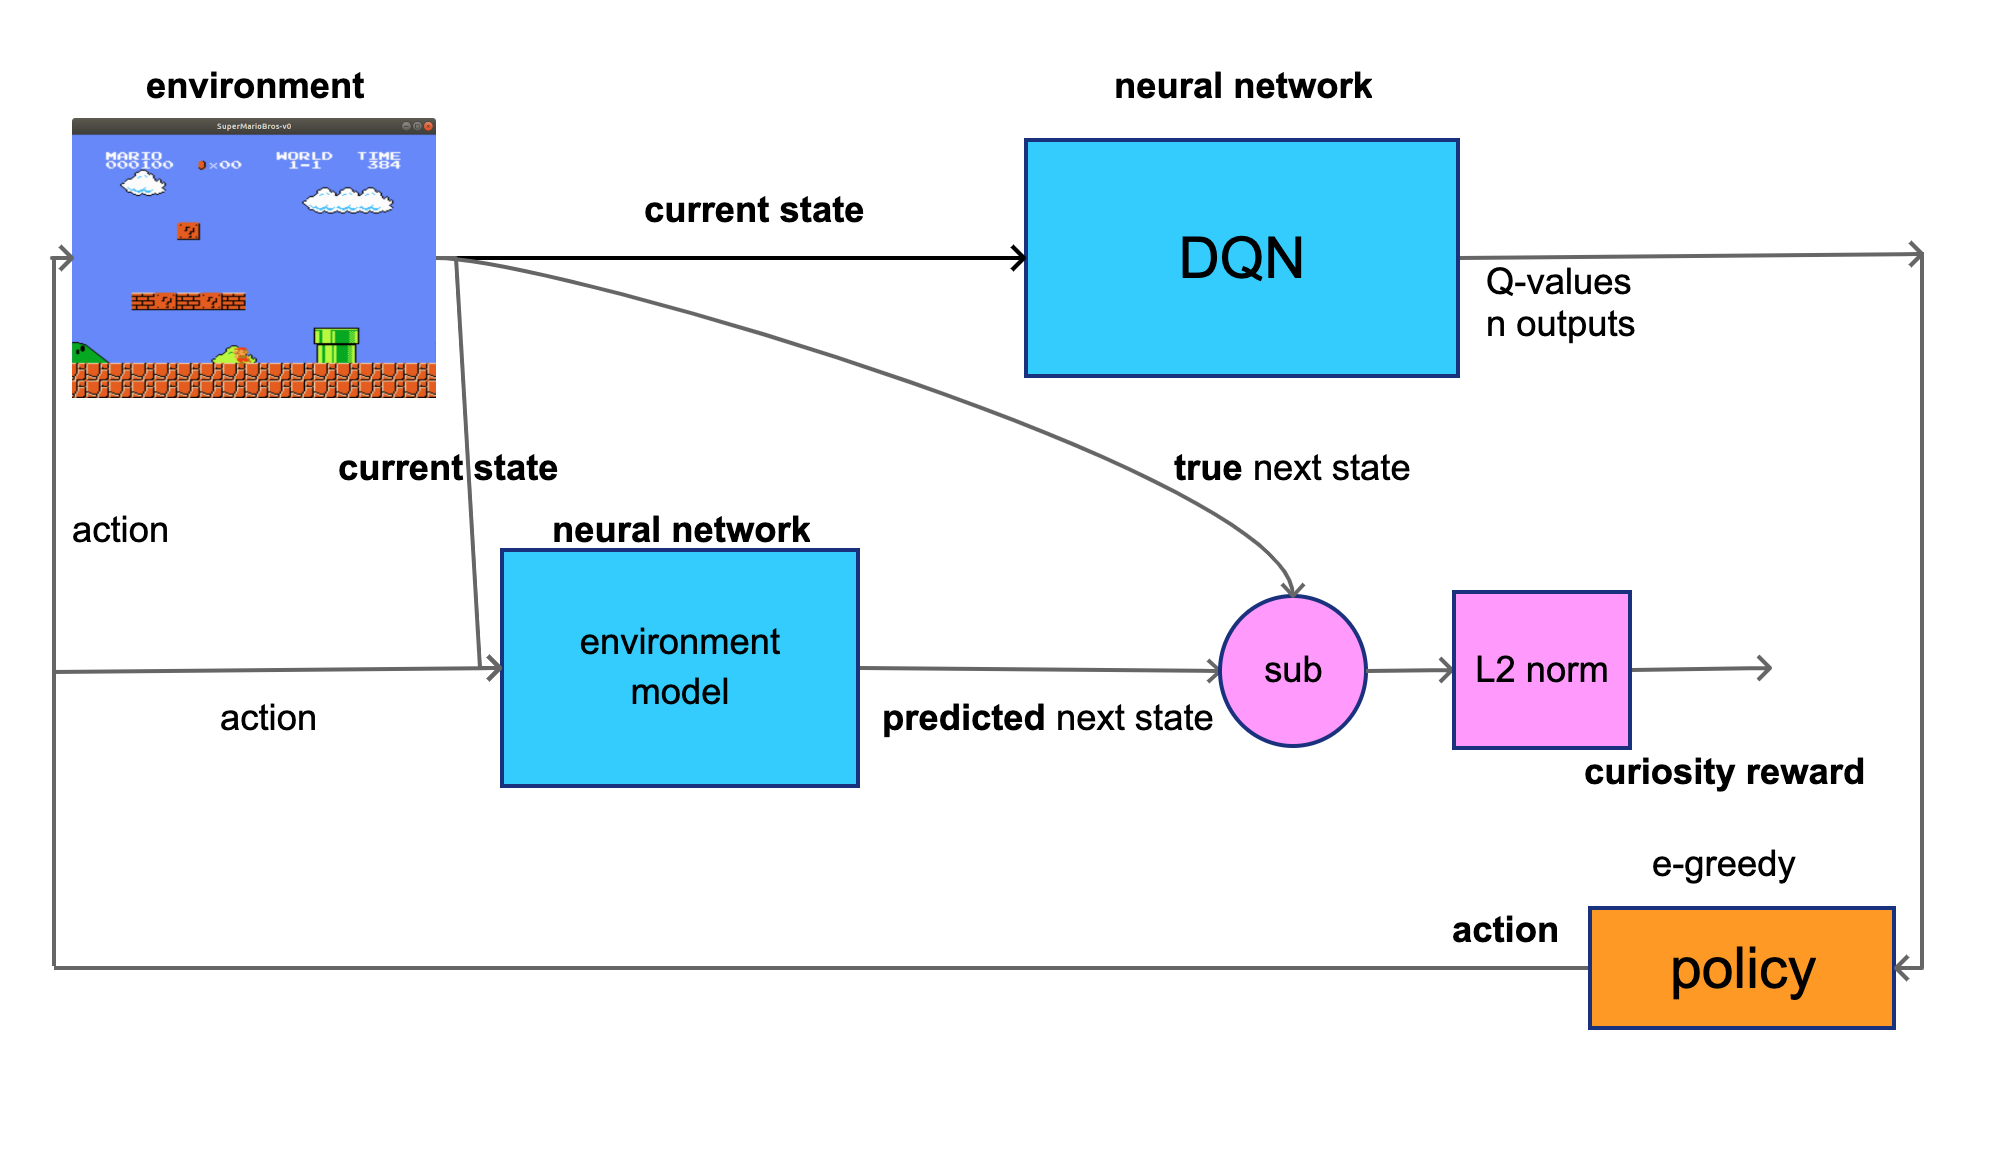
\includegraphics[scale=0.12]{../diagrams/dqncuriosity.png}}

  \begin{align*}
      Q'(s, a; \theta) &= R + \beta C(s, s', a; \phi) + \gamma \max \limits_{a'} Q(s', a'; \theta^-) \\
      \mathcal{L}_{em}(\phi) &= \left( s' - EM(s, a; \phi)  \right)^2 \\
      C(s, s', a) &= \Vert s' - EM(s, a; \phi) \Vert ^2_2
  \end{align*}

\end{frame}

\begin{frame}{\bf environment model - vector input}

  {\centering 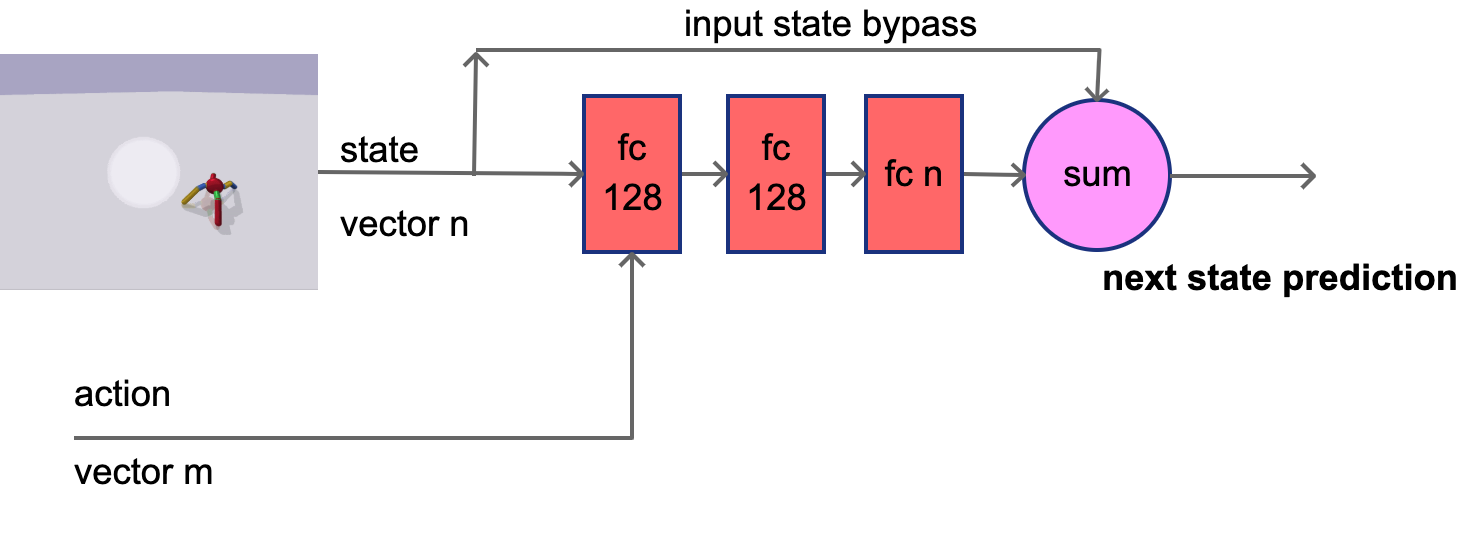
\includegraphics[scale=0.22]{../diagrams/fccuriositydetail.png}}

\end{frame}

\begin{frame}{\bf environment model - vector input}

  {\centering 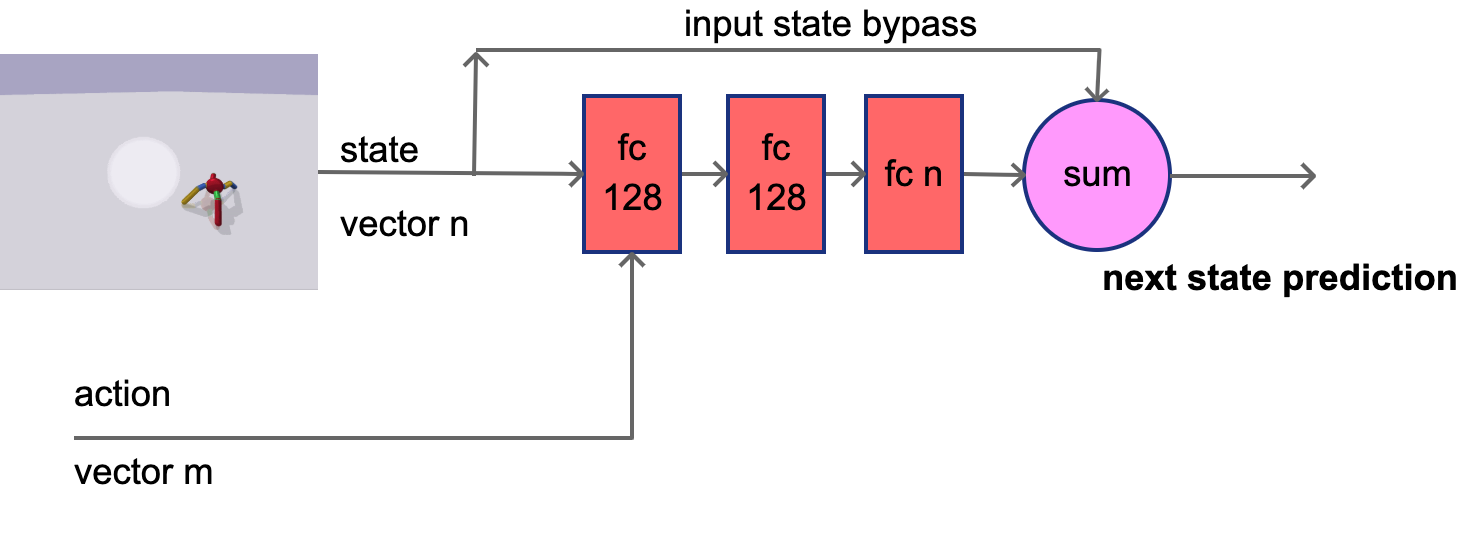
\includegraphics[scale=0.15]{../diagrams/fccuriositydetail.png}}
  {\centering 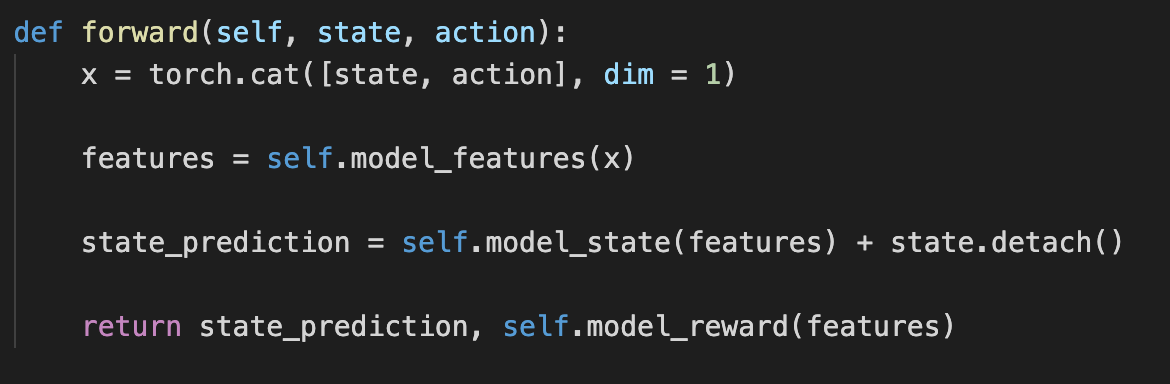
\includegraphics[scale=0.5]{../images/curiosity_fc.png}}

\end{frame}


\begin{frame}{\bf environment model - visual input}

  {\centering 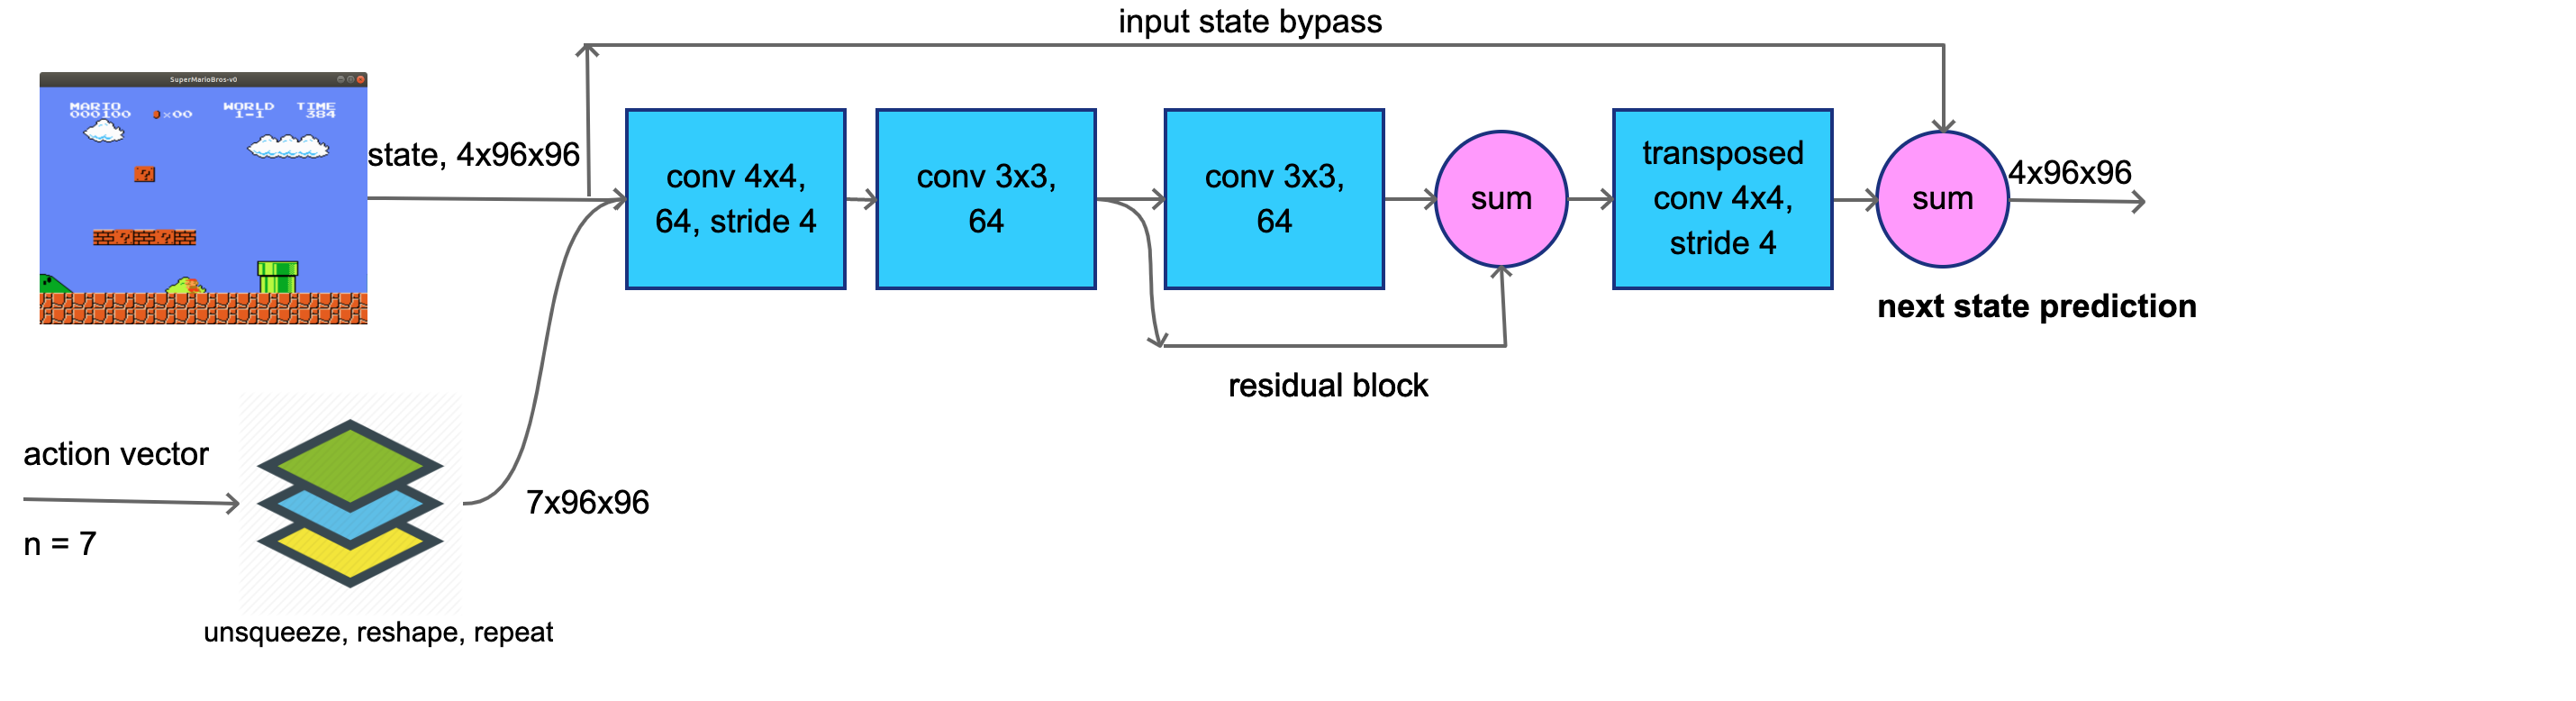
\includegraphics[scale=0.12]{../diagrams/convcuriositydetail.png}}

\end{frame}

\begin{frame}{\bf environment model - visual input}

  {\centering 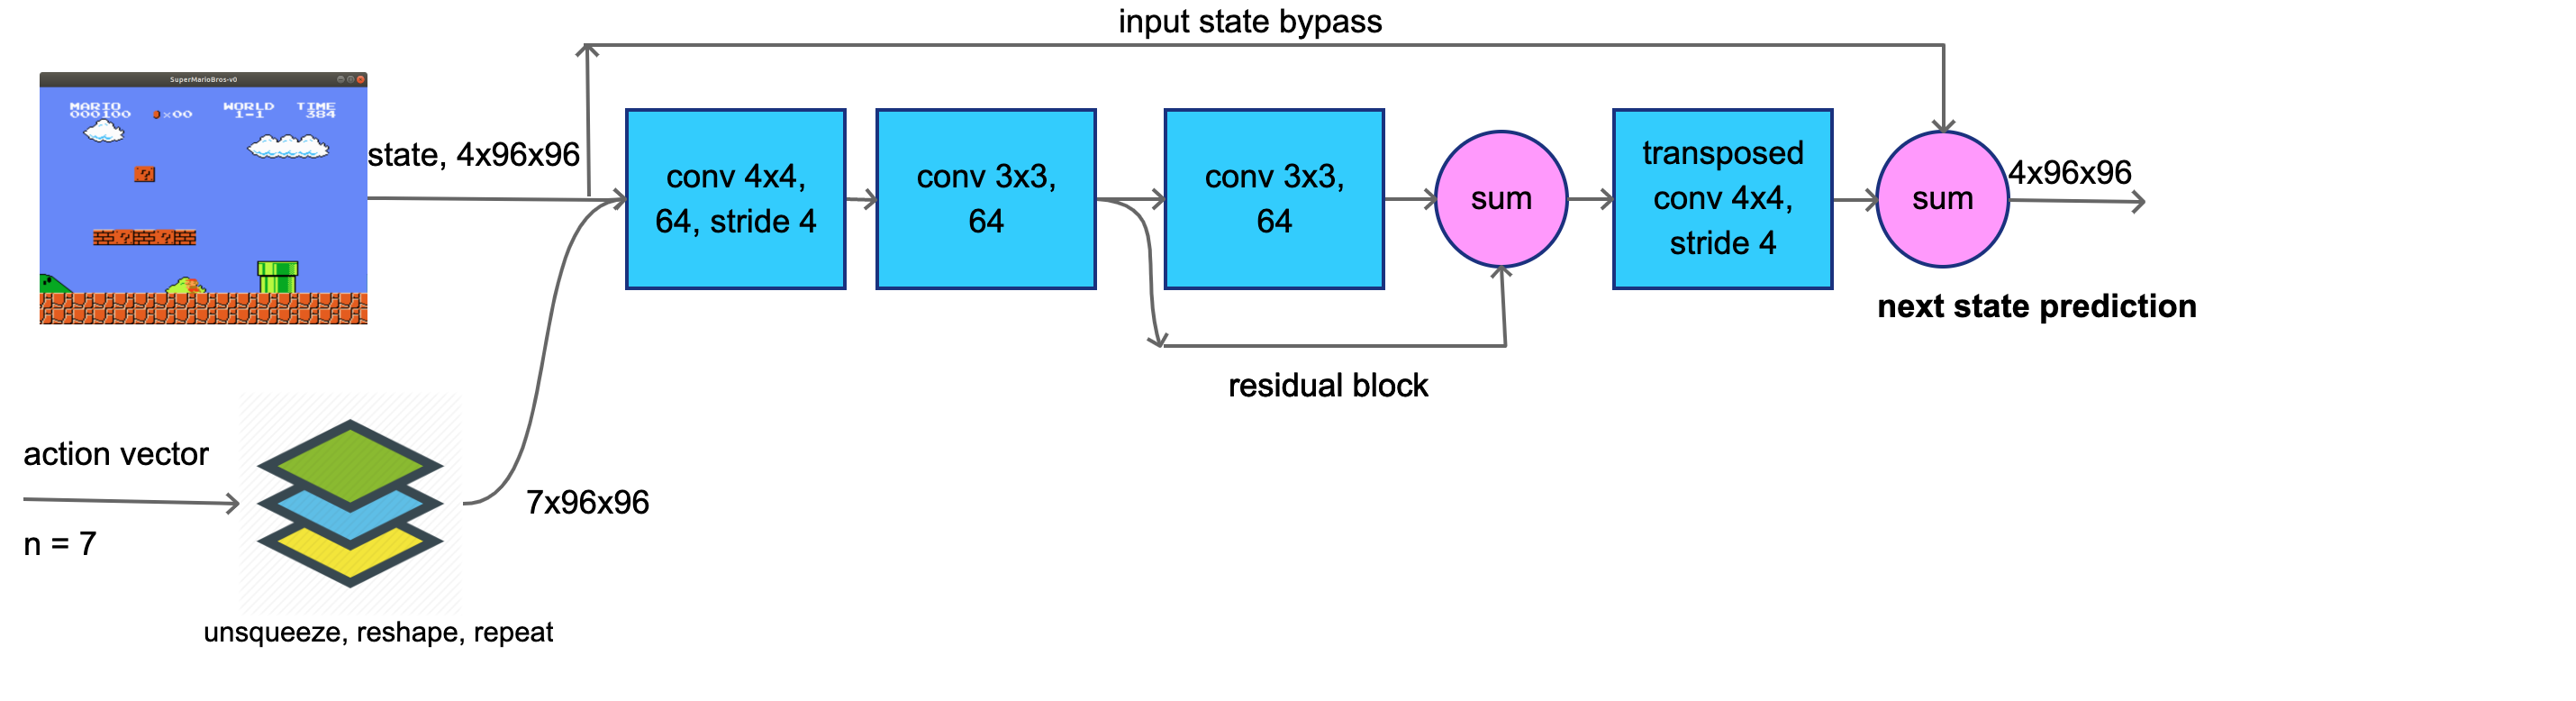
\includegraphics[scale=0.12]{../diagrams/convcuriositydetail.png}}
  {\centering 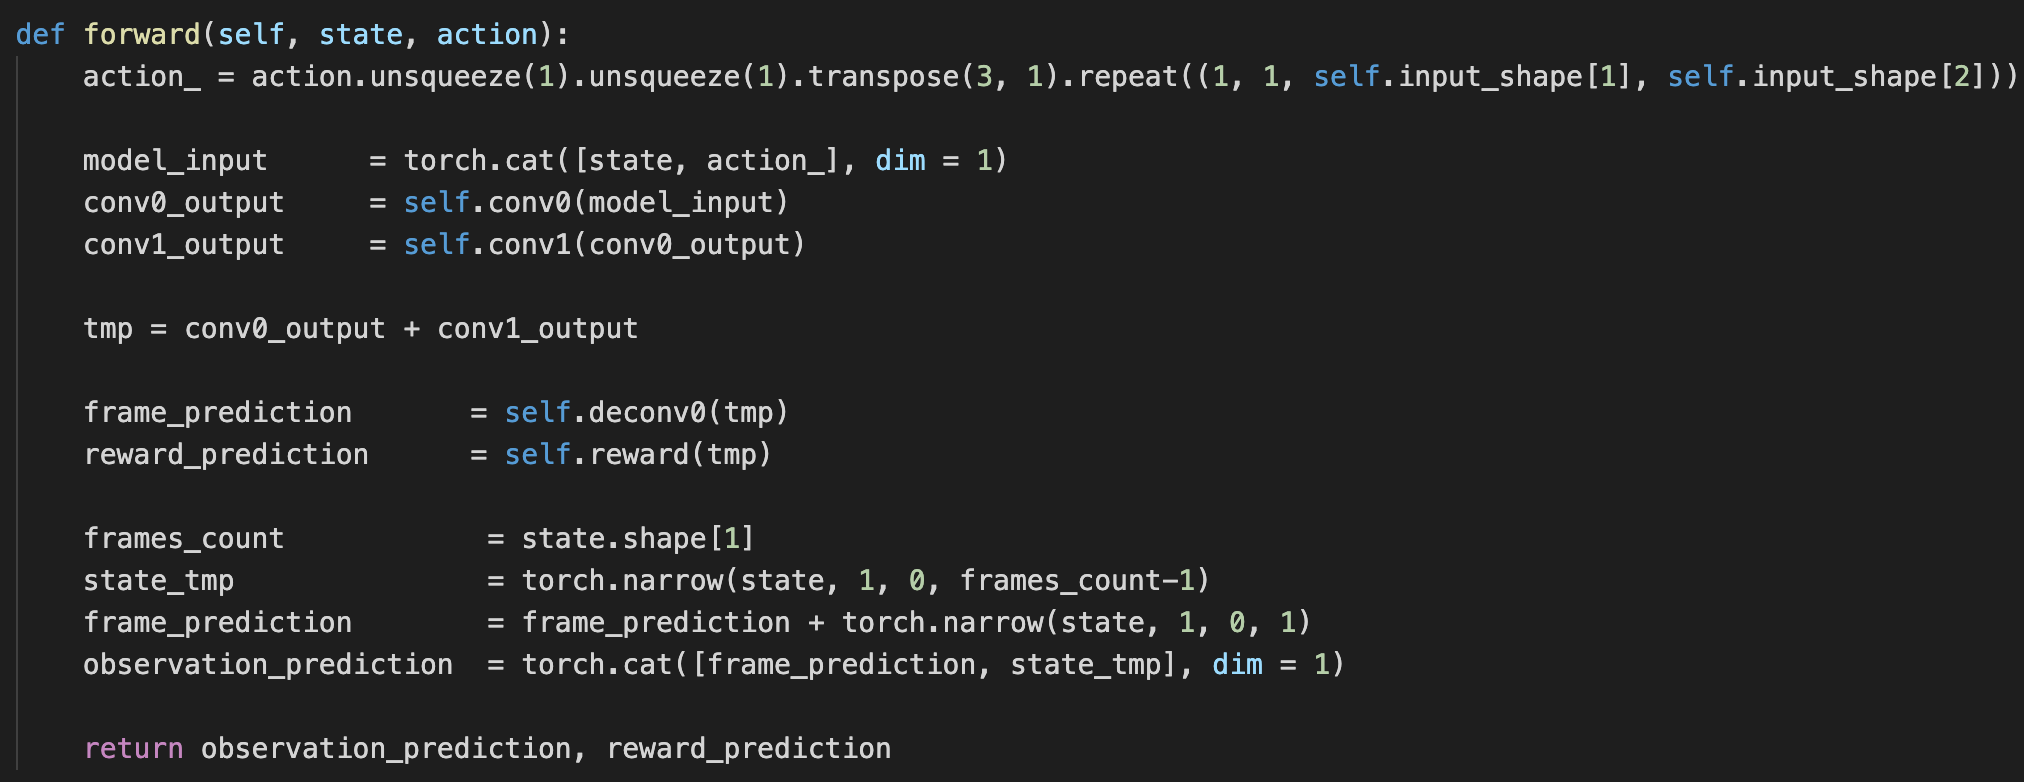
\includegraphics[scale=0.3]{../images/curiosity_conv.png}}

\end{frame}

\begin{frame}{\bf environment model - visual input}

  {\centering 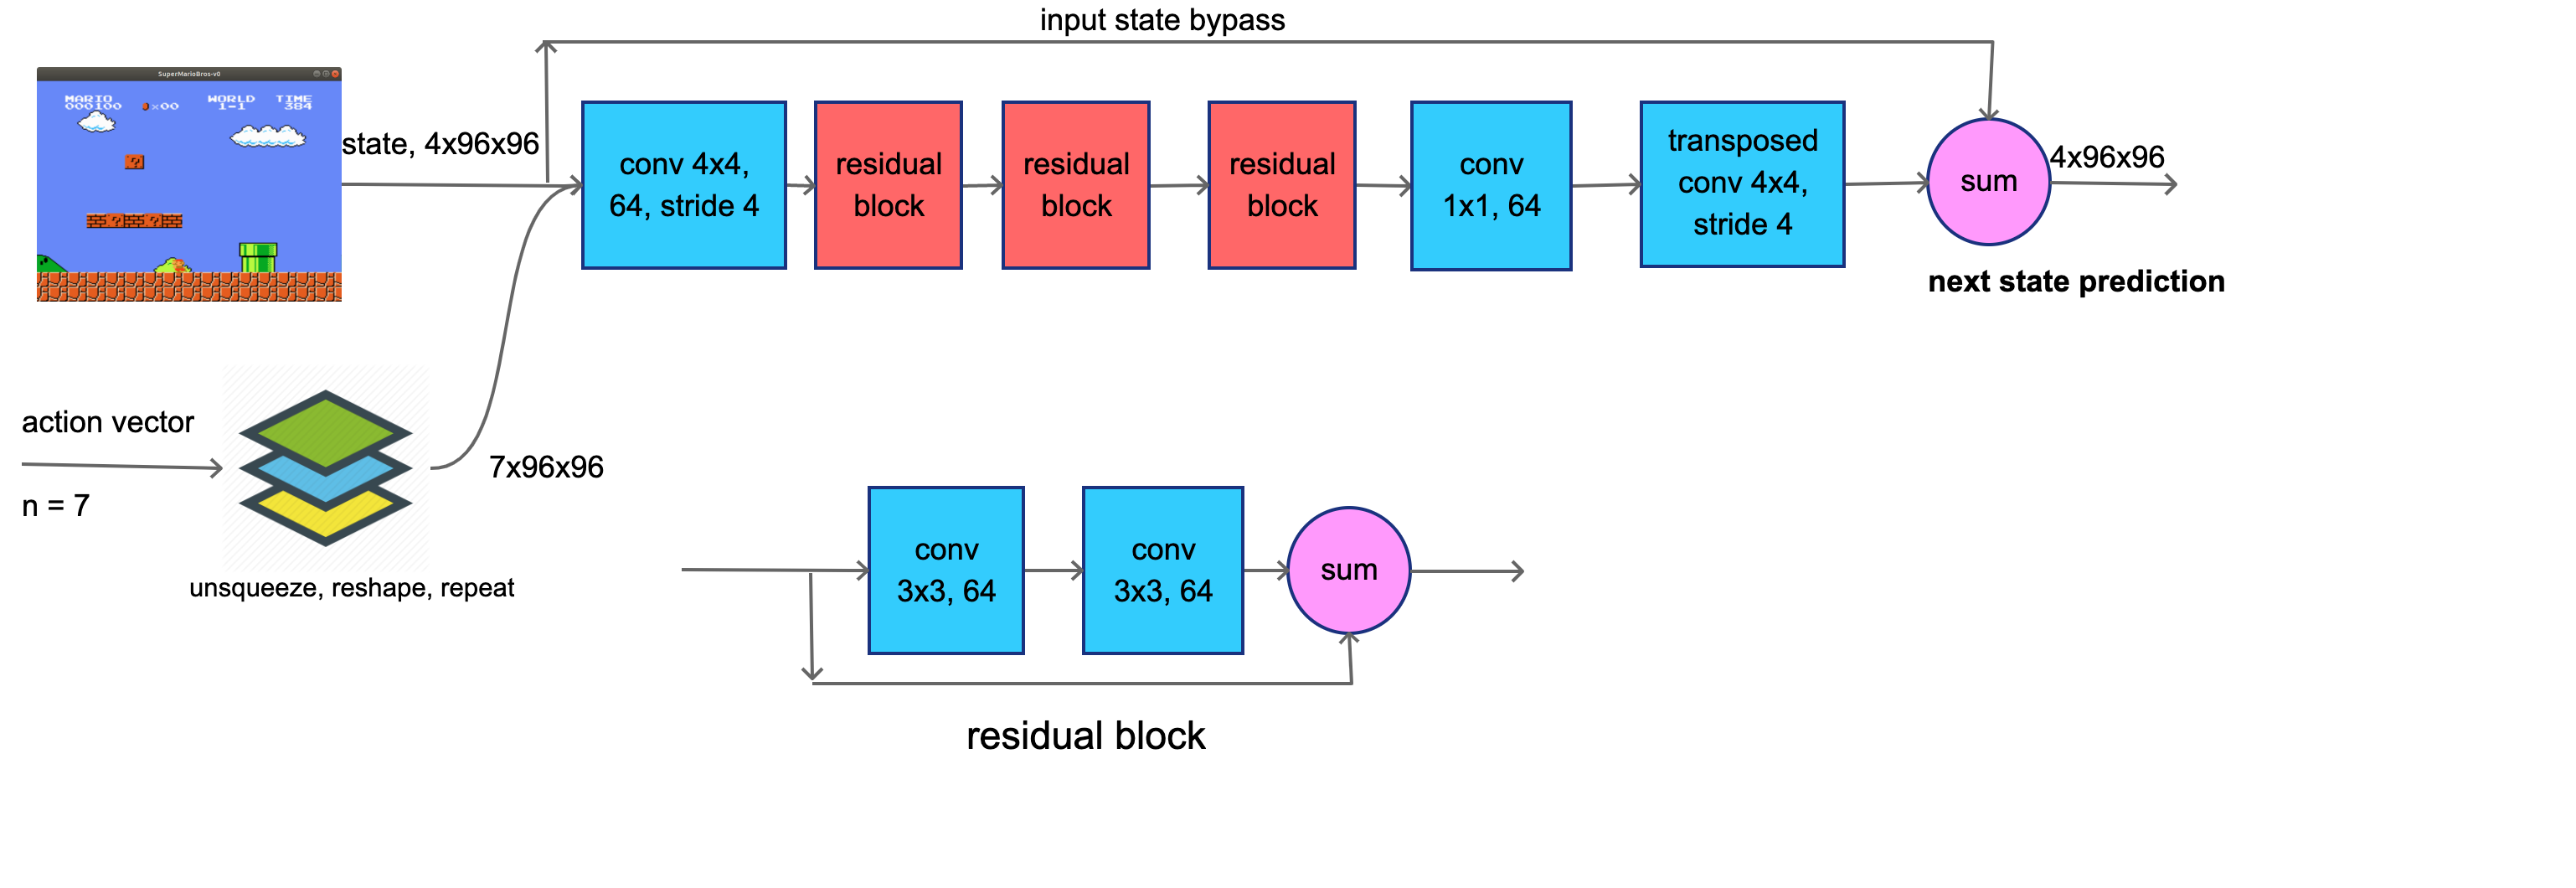
\includegraphics[scale=0.12]{../diagrams/convresnetcuriositydetail.png}}

\end{frame}


\begin{frame}{\bf imagination augmented agents}

  {\centering 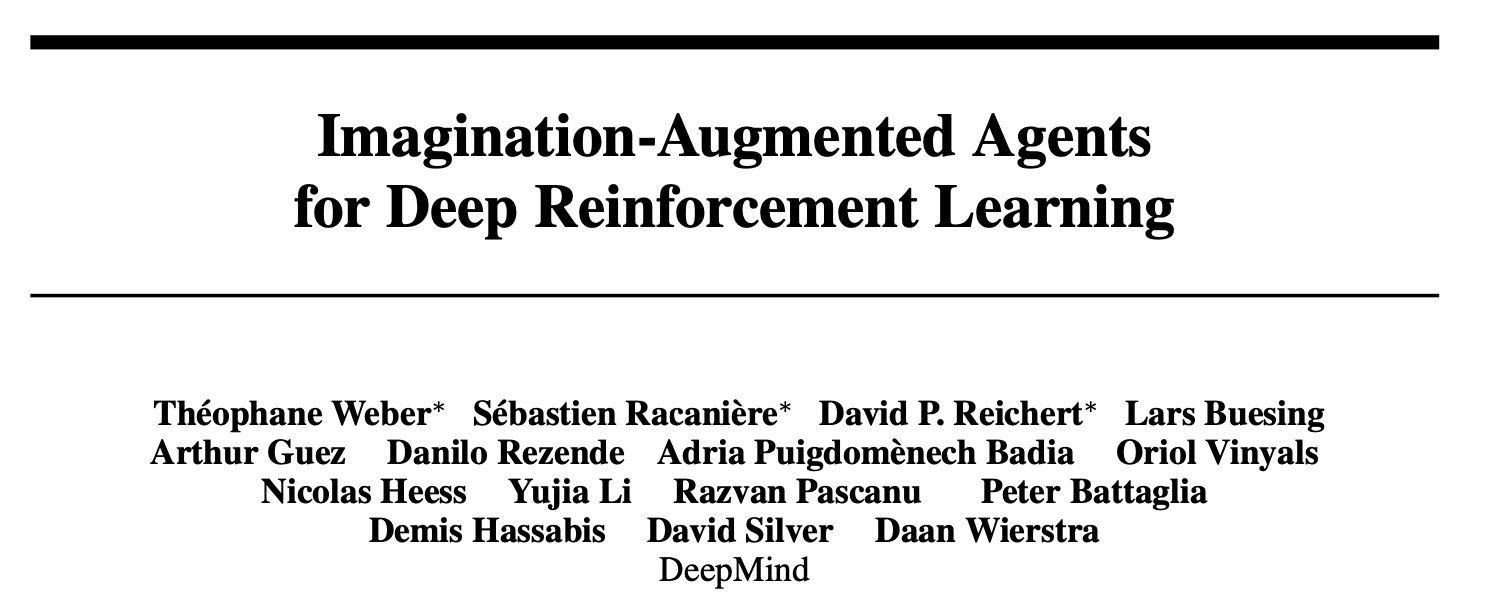
\includegraphics[scale=0.2]{../images/paper_imagination_0.png}}


  \begin{columns}

    \begin{column}{0.5\textwidth}
      \begin{itemize}
        \item imagination-Augmented Agents for Deep Reinforcement Learning, 2018, Theeophane Weber
        \item {\bf \color{red} main idea } : exploration and action selection in imagined trajectories first
      \end{itemize}
    \end{column}

    \begin{column}{0.5\textwidth}
      {\centering 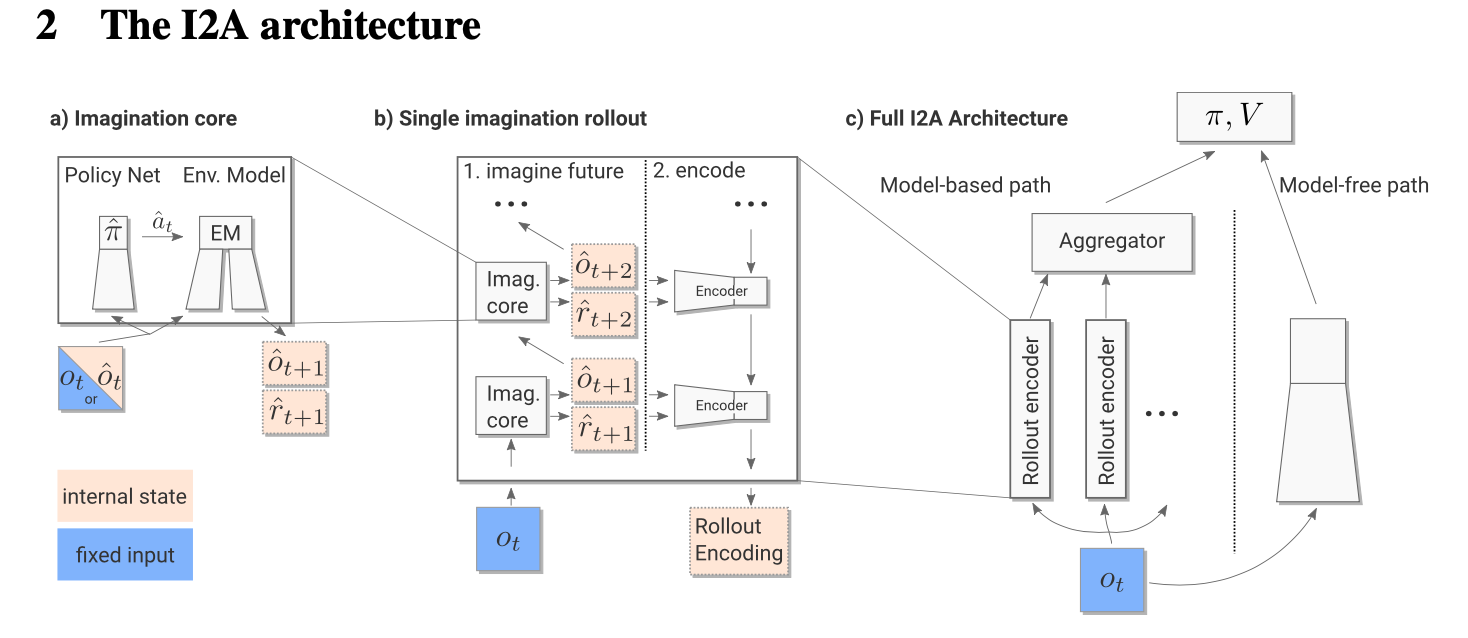
\includegraphics[scale=0.25]{../images/paper_imagination_1.png}}
    \end{column}

  \end{columns}


\end{frame}


\begin{frame}{\bf imagination in RL}

  {\centering 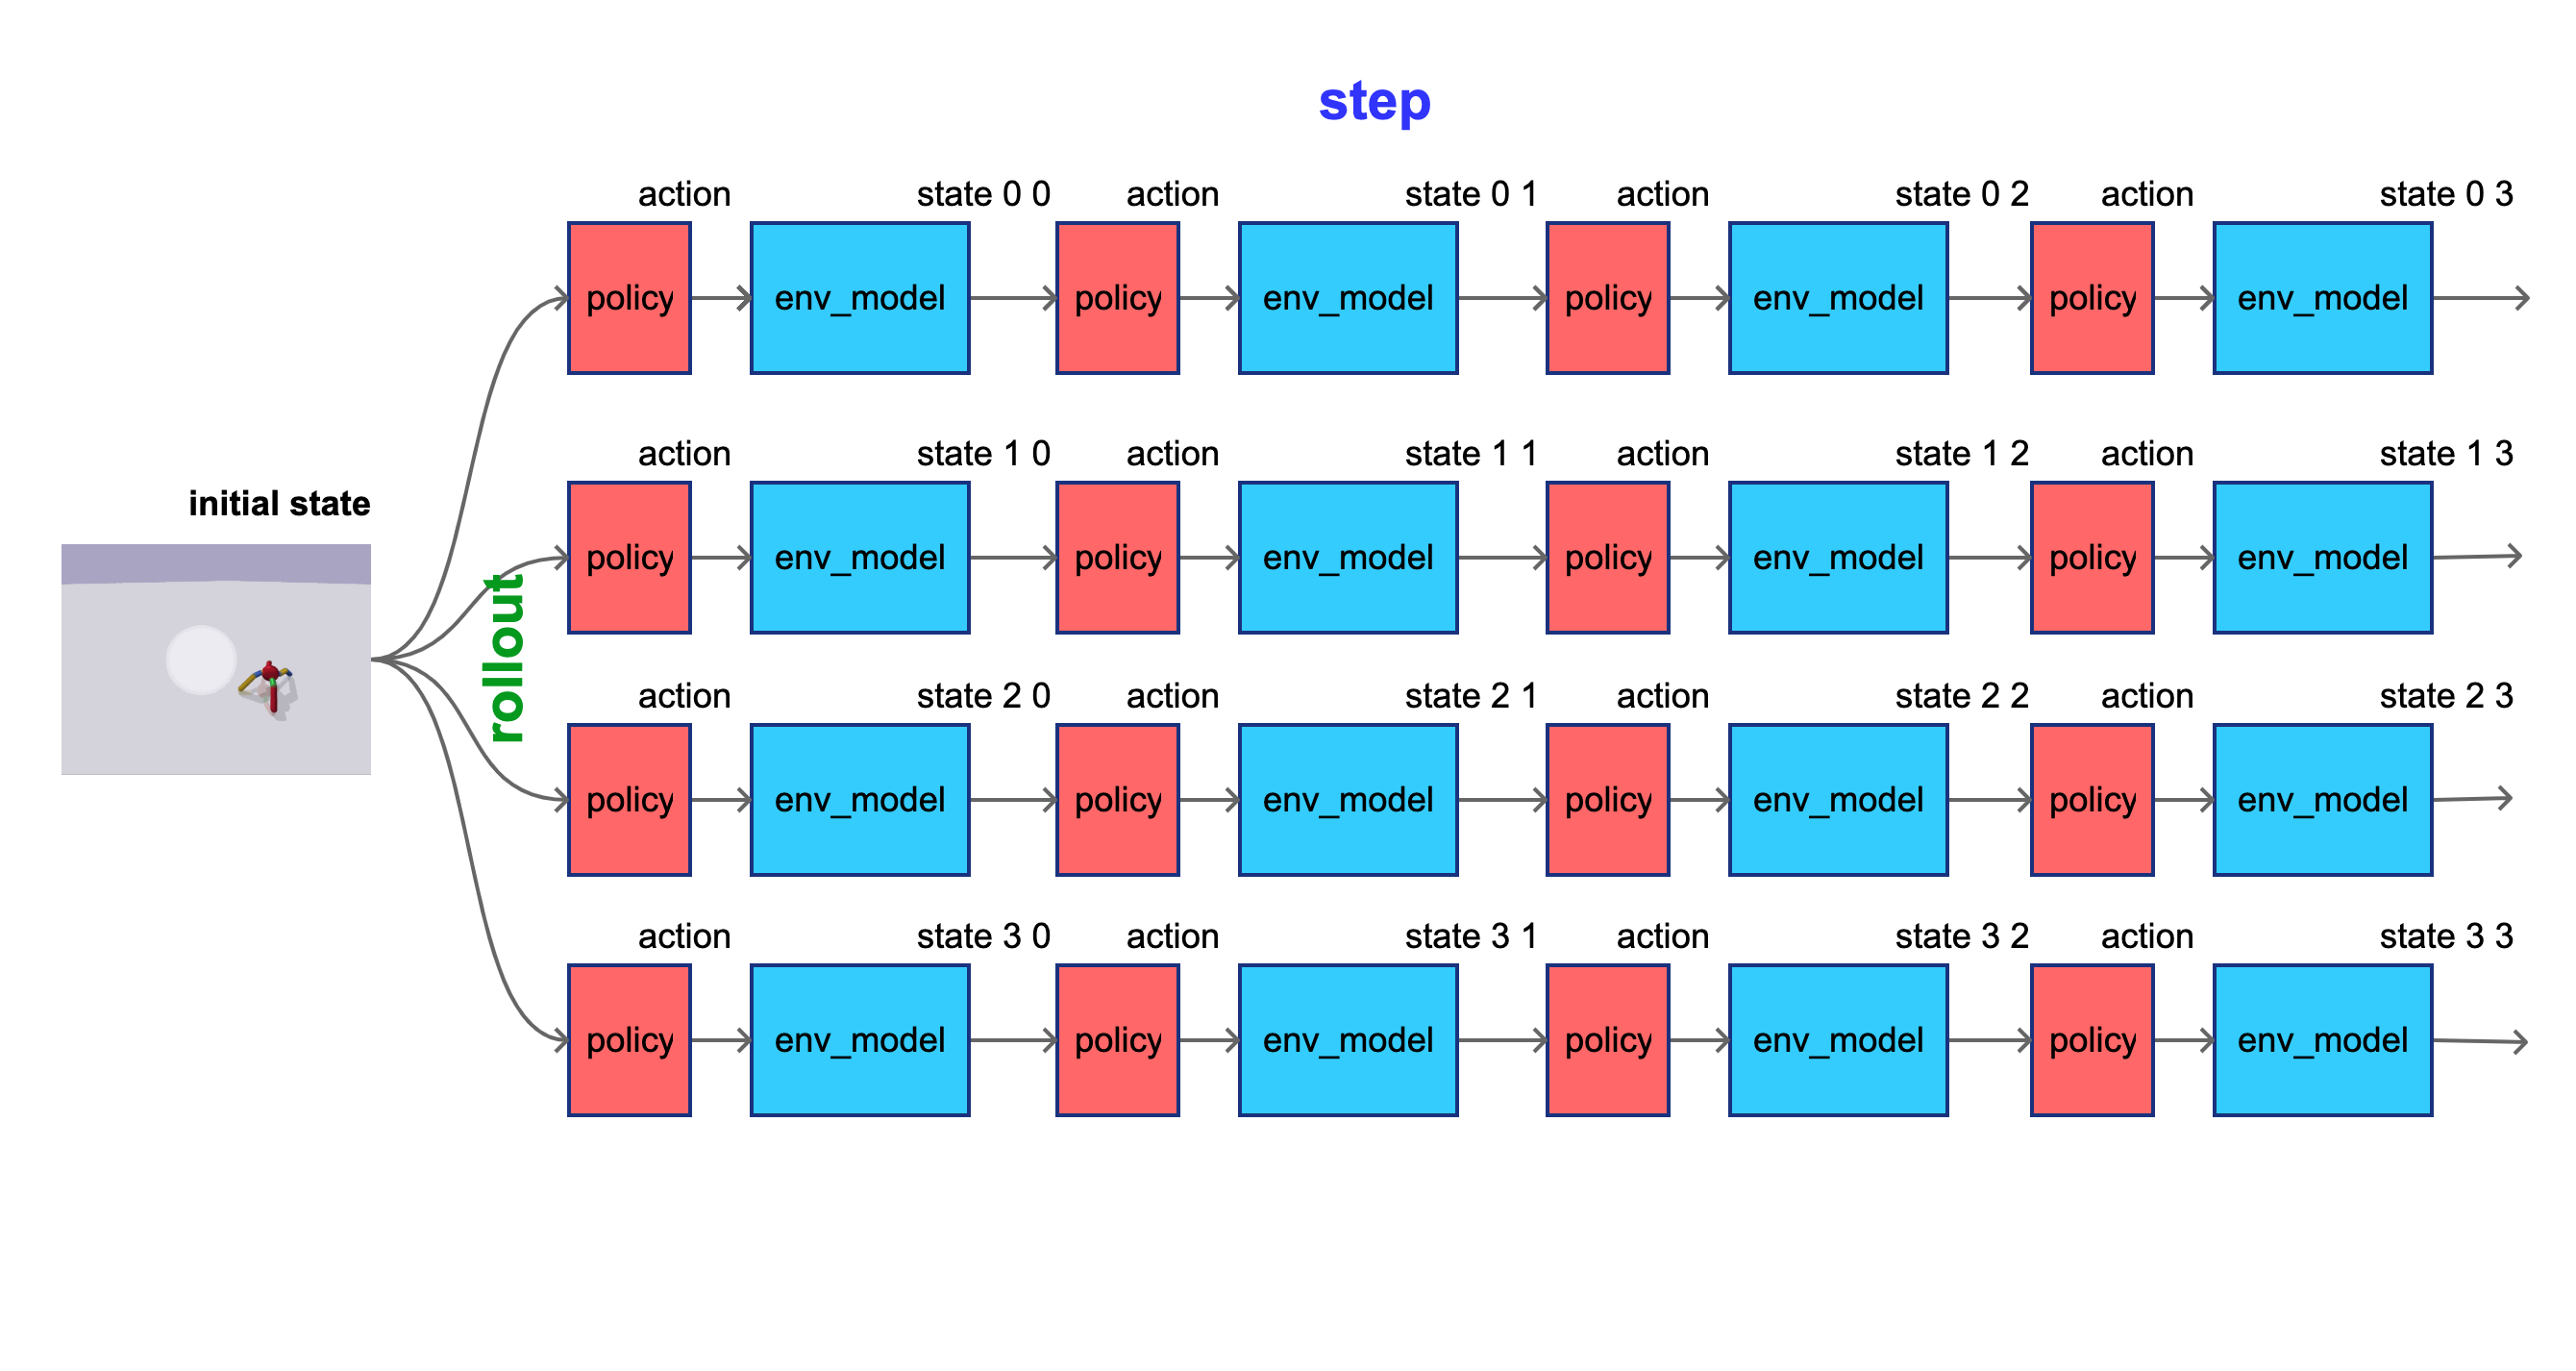
\includegraphics[scale=0.12]{../diagrams/imagination.png}}
\end{frame}

\begin{frame}{\bf imagination in RL - model detail with meta-actor}

  {\centering 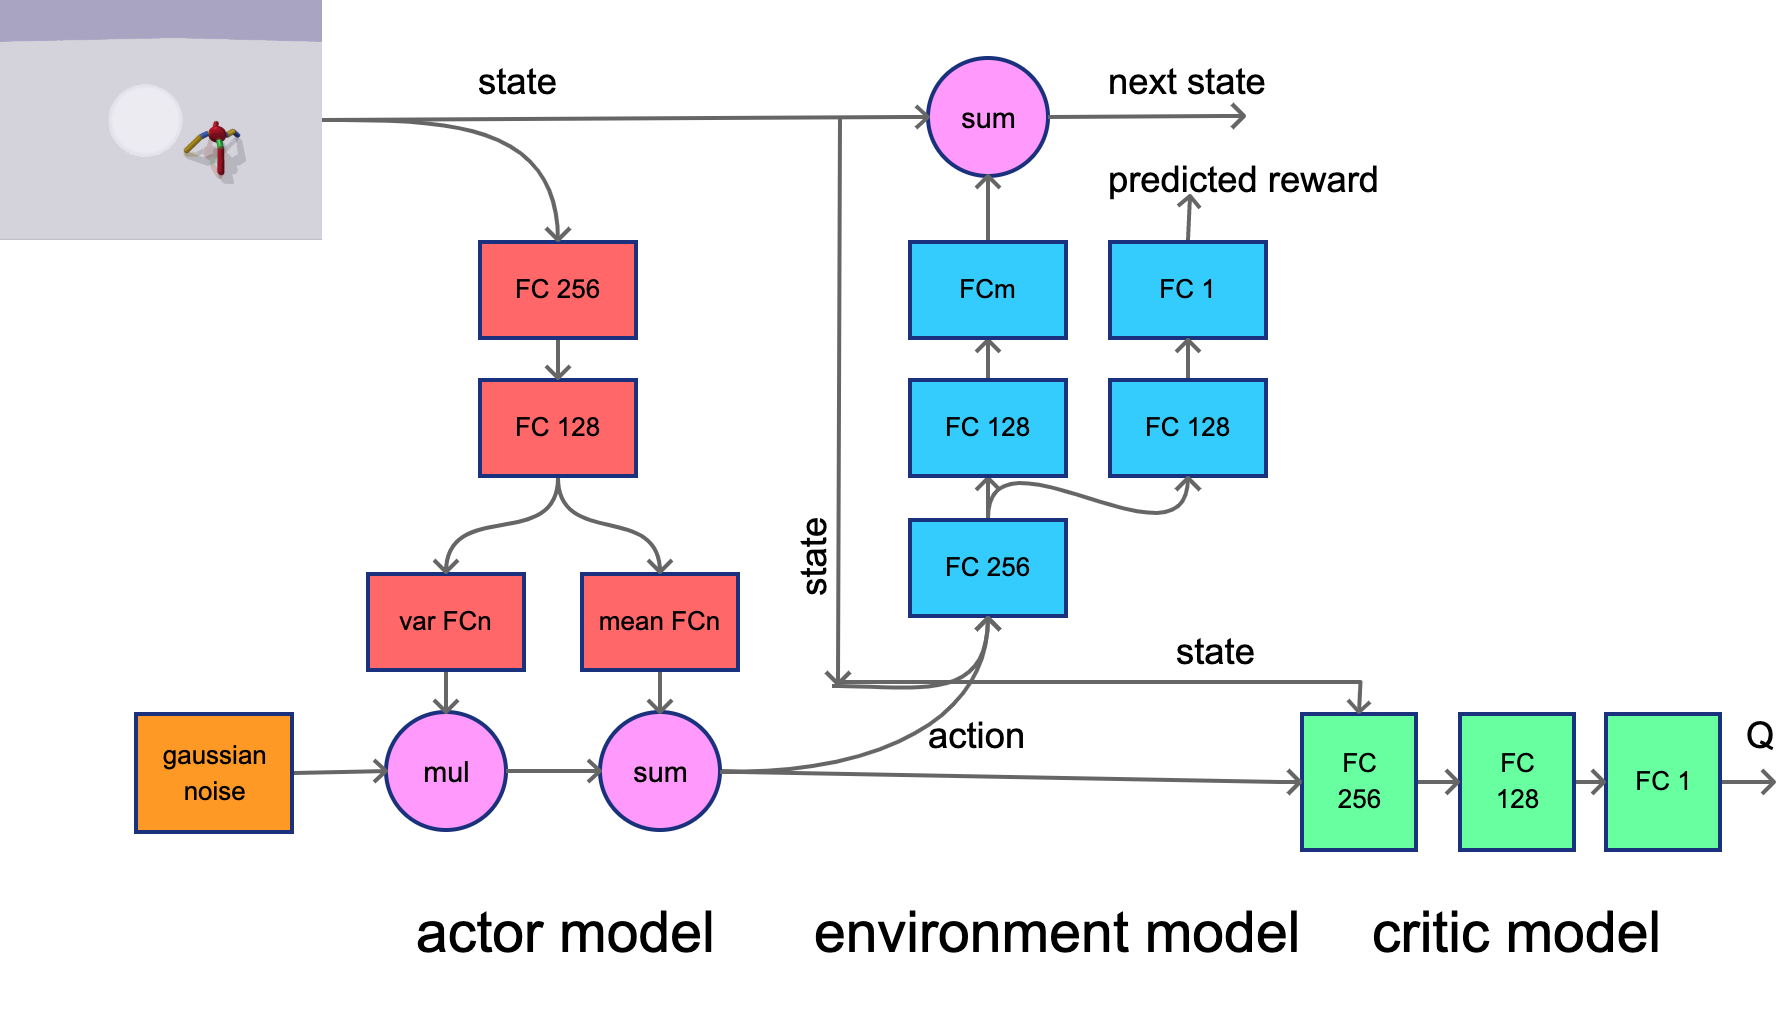
\includegraphics[scale=0.18]{../diagrams/imaginationmodeldetail.png}}
\end{frame}

\begin{frame}{\bf imagination in RL - model detail with meta-actor}

  {\centering 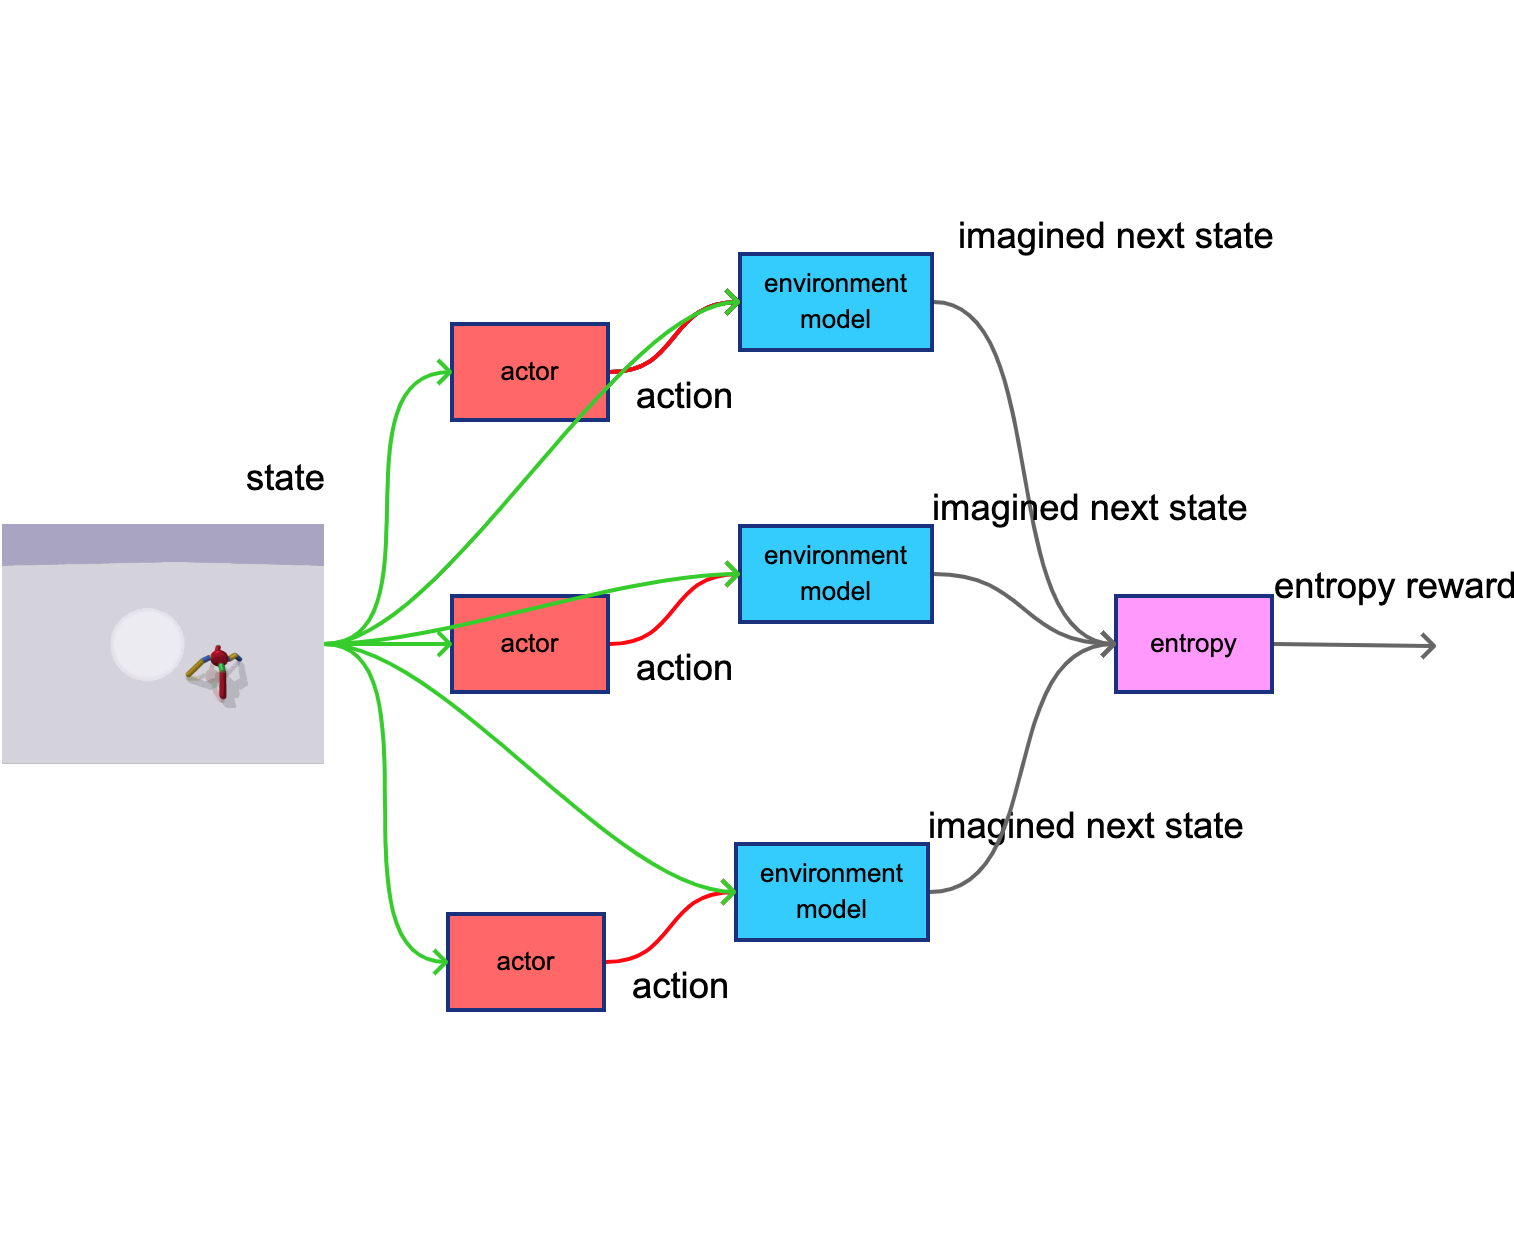
\includegraphics[scale=0.08]{../diagrams/imaginationentropy.png}}

  \begin{align*}
    \mathcal{L}_{entropy}(\phi) &= -\frac{1}{2} ln(2\pi e \sigma(.;\phi)^2)
  \end{align*}


  note : maximum entropy defined as
    \begin{align*}
      H(x) = \int_{-\infty}^{\infty} x ln(x)dx
    \end{align*}
\end{frame}



\begin{frame}{\bf imagination in RL - model detail with meta-actor}

  {\centering 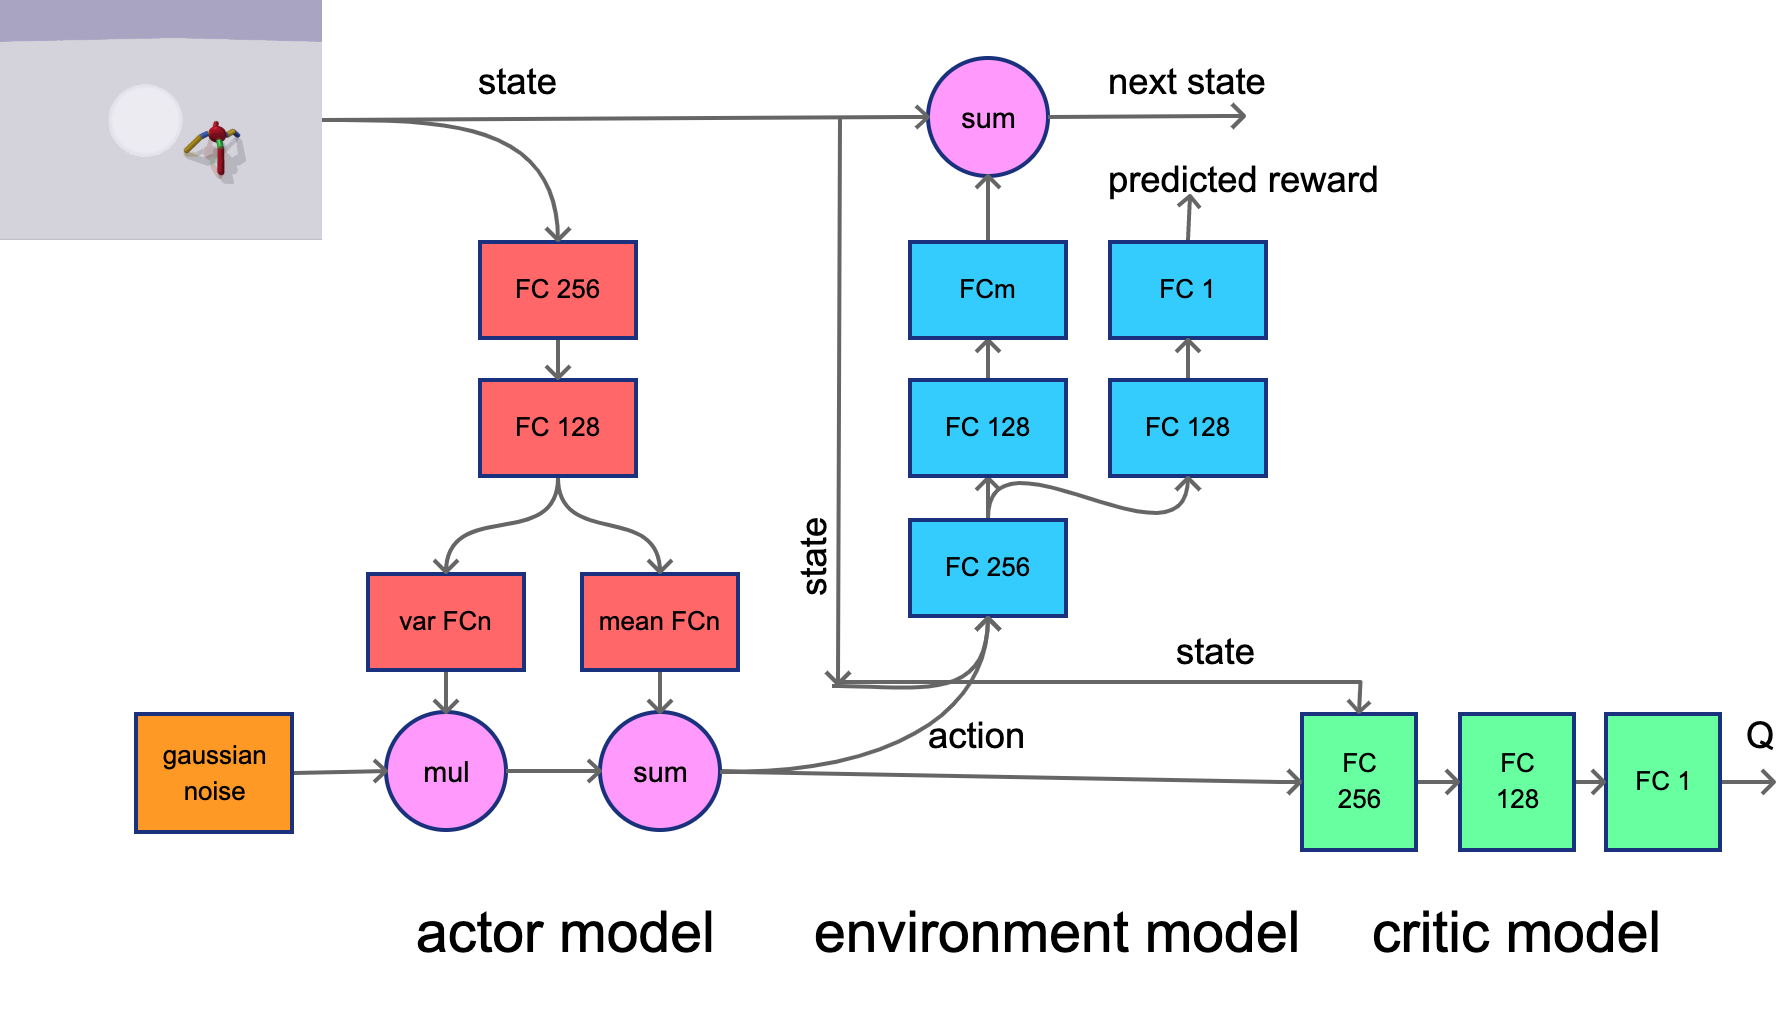
\includegraphics[scale=0.1]{../diagrams/imaginationmodeldetail.png}}

  
    \begin{align*}
      \mathcal{L}_c(\theta) &= \left( R + \gamma Q(s', a'; \theta^-, \phi^- ) - Q(s, a; \theta, \phi )  \right)^2 \\
      \mathcal{L}_a(\phi) &= -Q(s, a; \theta, \phi) - \beta H(\{s^{im}_0 .. s^{im}_k\}; \phi) \\
      \mathcal{L}_m(\kappa) &= \left( s' - EM(s, a; \kappa)  \right)^2 \\    
    \end{align*}
\end{frame}


\begin{frame}{\bf books to read}

\begin{itemize}
  \item Maxim Lapan, 2020, Deep Reinforcement Learning Hands-On second edition
  \item Maxim Lapan, 2018, Deep Reinforcement Learning Hands-On
  \item Praveen Palanisamy, 2018, Hands-On Intelligent Agents with OpenAI Gym
  \item Andrea Lonza, 2019, Reinforcement Learning Algorithms with Python
  \item Rajalingappaa Shanmugamani, 2019, Python Reinforcement Learning
  \item Micheal Lanham, 2019, Hands-On Deep Learning for Games
\end{itemize}


\end{frame}

\begin{frame}{\bf Q\&A}

{\centering 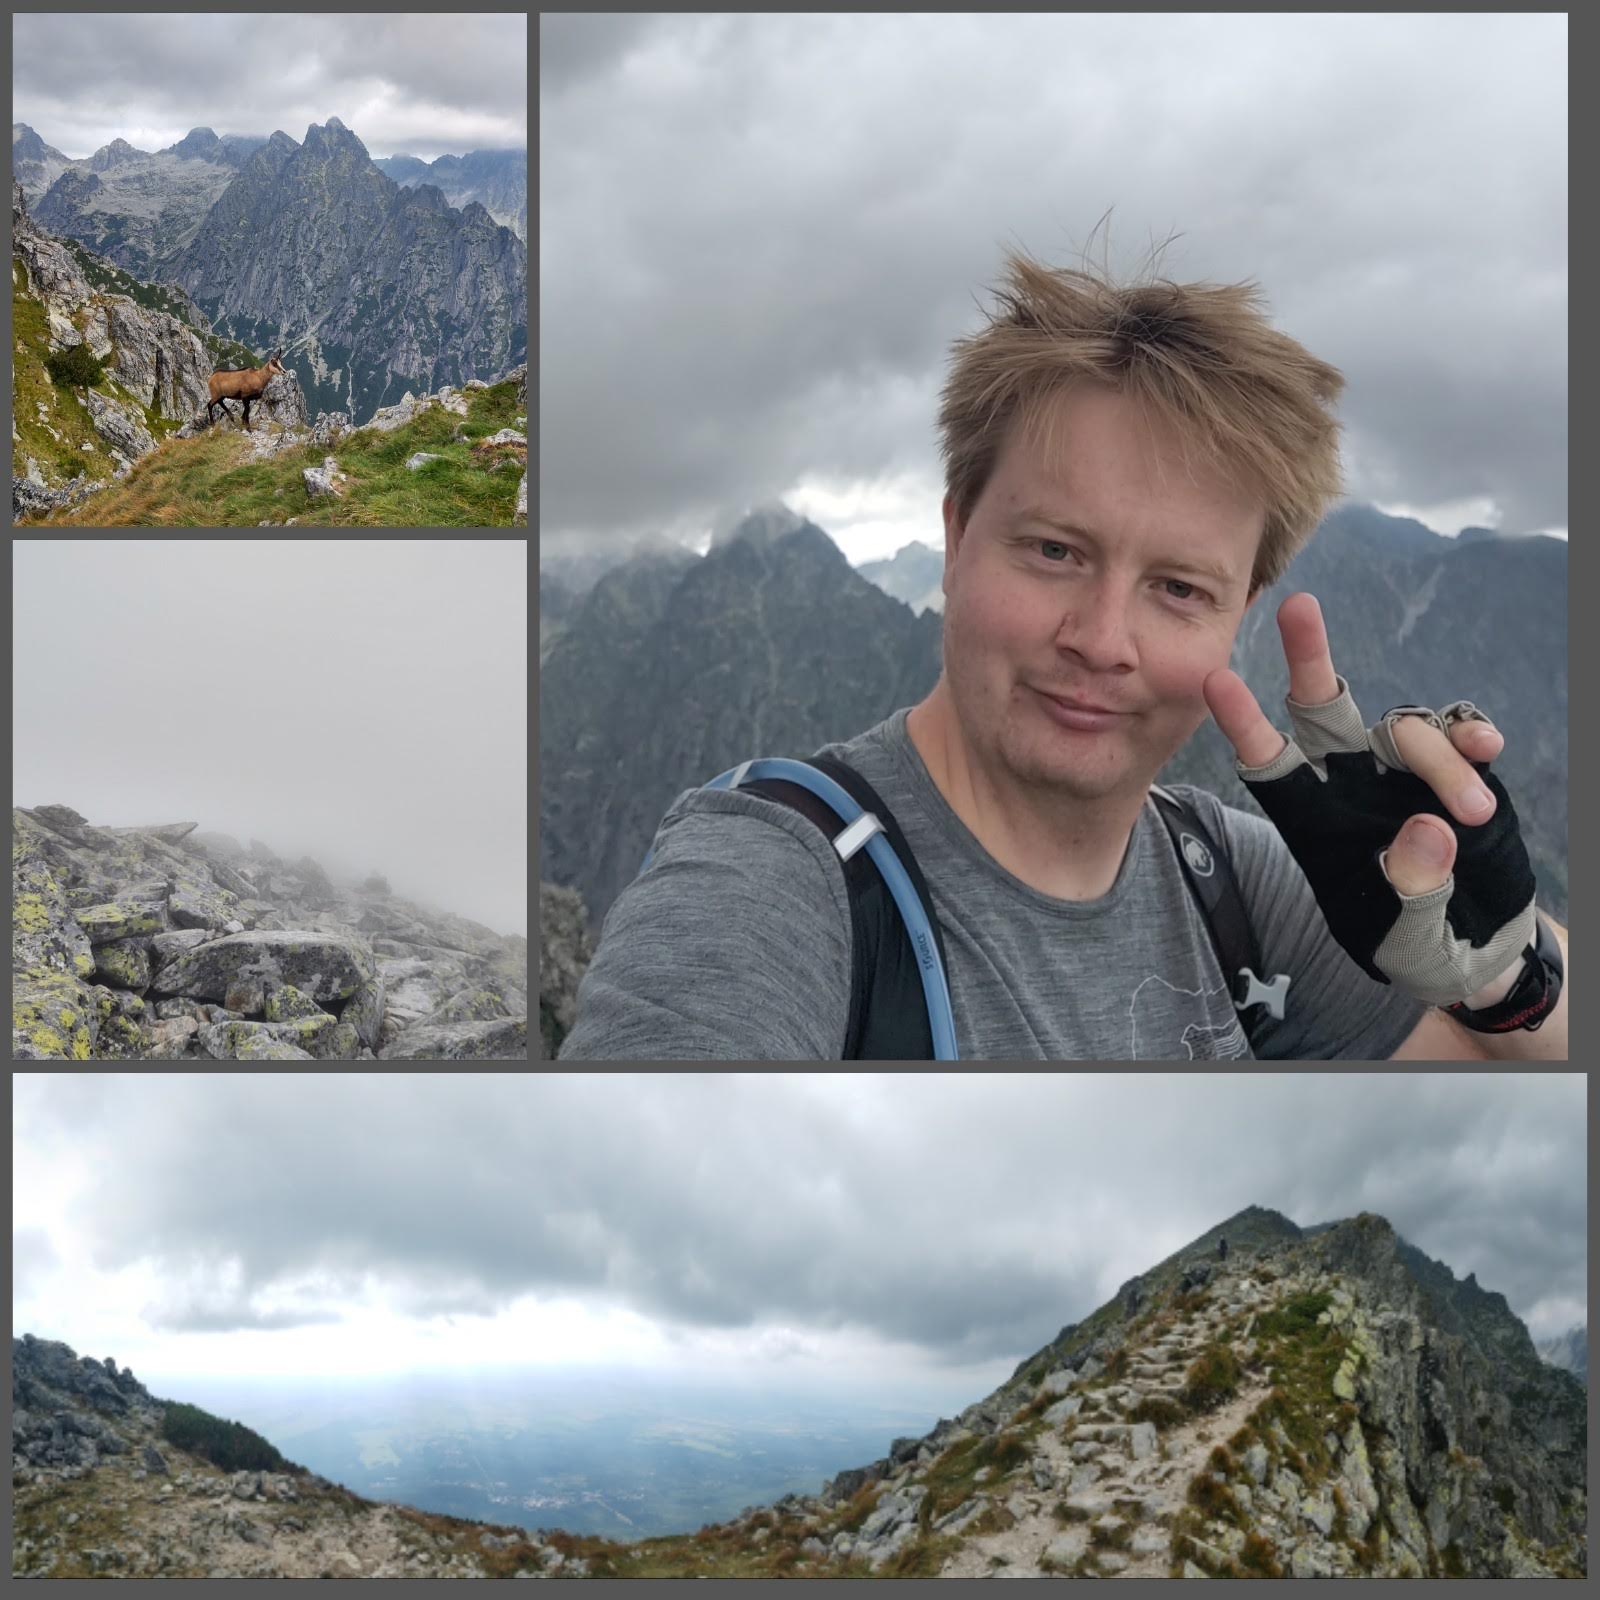
\includegraphics[scale=0.1]{../images/me.jpg}}

\url{michal.nand@gmail.com}

\url{https://github.com/michalnand/imagination_reinforcement_learning}

 
\end{frame}


\end{document}
